%\chapter{Neural Fields as Control and Planning Systems} 
\label{ch:chp2}
\section{Introduction}
\emph{The contents of this chapter were published, in two parts, in
  the Proceedings of the International Joint Conference of Neural
  Networks (IJCNN) 2009 and the Genetic and Evolutionary Computation
  Conference (GECCO) 2009.}

Artificial life aims to devise and study those emergent phenomena that
give complex attributes to the living beings, like self-organization,
cooperation, self-reproduction and adaptation, among others
\cite{Bedau92Philosophical}. It focuses on the generation of behavior
from a biological, bottom-up perspective that relies on evolution,
development and learning \cite{Dyer94Toward}.

Following a pure artificial life approach to evolutionary robotics
\cite{Nolfi04Evolutionary}, it is expected that complex behaviors of
simulated agents emerge by local interactions of elements. These
interactions form a complex dynamical system which is the generator of
behavior and is capable of some form of adaptation or
evolution. Examples of such dynamical systems are recurrent neural
networks \cite{Huelse04Structure} and feed-forward neural networks
\cite{Stanley02Evolving}.

One of the tasks in evolutionary robotics is the emergence of motion
control and planning capabilities of biped walking agents.

In biped robotics, the methods based on computational intelligence for
planning and control have shown to be able to achieve static stability
\cite{Kun97Adaptive}, dynamical stability
\cite{Nakanishi2004b,Komatsu05Dynamic}, achieve simple control
structures \cite{Huelse04Structure}, and tolerate perturbations
\cite{Juang02Intelligent}. Nonetheless, those properties have not been
extended to an integrated architecture of planning and control capable
of following goals (for details see the previous chapter).

Here, there are compared two control schemes based on neural networks
in order to observe their advantages and disadvantages as planning and
control architectures and their suitability as controllers given their
structure. The first one, uses a simple model of recurrent connections
between neurons without additional restrictions, i.e. a recurrent
neural network. The second one, based on neural fields, has a deeper
biological basis, applies more restrictions and extends the discrete
model to a continuous one, following the method of planning and
control by means of neural fields \cite{Bergener99Complex}. The neural
field model, as noted in the article by Bergener et al., has the
potential to address goal-based planning problems, so we are here
interested on its capability to solve dynamic control problems.

The control problem set for testing the architectures is the stability
problem on a inverted pendulum, so that the controller ability to
perform dynamic control on an unstable plant can be evaluated. This is
a first attempt (to the authors' knowledge) to evaluate neural fields
for solving a control problem for an unstable plant, and specifically
for solving the inverted pendulum control problem. However, there is a
wide range of methods that have been applied to the inverted pendulum
problem both based on computational intelligence
(e.g. \cite{Anderson89Learning, Bardossy95Fuzzy, Moriarty96Efficient,
  Zhang02recurrent}) and based on control theory techniques
(e.g. \cite{Kajiwara99LPV, Huang00Control, Chang02self-tuning}).

In this chapter we aim to propose a control planning system or
architecture based on neural fields which is suitable to control a
relatively complex system. We test it over the stability problem on a
typical inverted-pendulum and compare it against a more traditional
recurrent neural network controller. First, we present the neural
fields model, some variations of it which will be useful for its
evolution and some of the properties that arise from it. Next, we
study its applications to control and compare it with the recurrent
neural network control scheme. We briefly compare its properties with
traditional control schemes, and then we test it with the
inverted-pendulum problem. Finally, we show how evolution algorithms
are applied to the neural field, and discuss the results obtained.

% \section{Goal-Based Planning and Control Planning}

\section{Neural Fields for Control and Planning}
For the purpose of control and planning we need some particular
requirements on the neural fields.

The first one is to have a preprocessing over the input
obtained from the sensors, so that there is a closed loop where the
representation of inputs has an appropriate form. This mechanism alone
(a particular form for the inputs) has shown to be enough for the robot
ARNOLD to navigate in the plane with obstacles
\cite{Bergener99Complex}.

The second one is to be able to modify the connection kernel so that
it can be suitable to our control problem. In order to do that, we
will consider that the connection kernel $w(y)$ is a symmetric
function (i.e. $w(y)=w(-y)$), that also is a 2-power Lebesgue
integrable function so that it also belong to $L^2$. It can be shown
that, with that definition, a sum of an arbitrary number of kernel
functions will also be a kernel function. This way, we have a
inner-product defined by the Lebesgue measure:

\begin{equation}
  \label{eq:eq-l2}
  \langle f,g \rangle_{L^2} = \int_{\mathbb{R}}{f\cdot g d\mu}
\end{equation}

The defined space, with its measure, conforms a Hilbert space, and
therefore is complete and metrizable. It also gives a notion of sum,
and scalar product:

\begin{align}
  \label{eq:eq-leb-opers}
  (f+g)(x)&=f(x)+g(x) \\
  (\lambda f)(x)&=\lambda f(x)
\end{align}
Those properties will be used shortly, when arises the problem of
kernel evolution.

The third one consists of its suitability to simulation. This is not an
inherent restriction for it to be physically (or biologically)
plausible, but to be implementable on a computer. We will take a
discrete form of the equation \ref{eq:nf-simp}:

\begin{equation}
  \label{eq:nf-disc}
  \tau \dot{u}_i=-u_i+\sum_{x_j \in B_p(x_i)} {w\left(x_i,x_j\right)
    f\left( u_j \right)}+S(x_i,t)
\end{equation}

Where we replace the integral for a sum over the point included inside
a finite neighborhood (ball) around $x_i$ with radius $p$. The time is considered
continuous, and the computation of the dynamical system behavior is
evaluated with a Runge-Kutta method. We denote $u_i=u(x_i,t)$. It
should be noted that the previous equation can be applied to the
$n$-dimensional case without modification.

\section{Control Architecture}
The control architecture built based on the neural fields has three
basic elements.

The first one, is a sensor, which reads the states from the plant and
also their derivatives (computed from the dynamical equation of the
plant). In particular, the sensor used for the neural field controller
is based on the angular acceleration of the pendulum pole, loosely
resembling the vestibular system on the inner ear.

The second one is the input layer, which consists of a simple neural
field without natural dynamics, where the spatial codification of the
sensed values is made. For the problem at hand, we use a finite
one-dimensional neural field, where a sensed input with value zero
maps to the center point of the field.

The third one is the processing layer, which has a more typical neural
field which has inner dynamics given by the eq. \ref{eq:nf-disc},
where the fields taken into the sum are the input neural field, and
the processing neural field. This way, besides its natural dynamics,
the processing layer receives the inputs from the input field filtered
by the kernel operator.

The parametrization of the controller is performed by varying the
kernel operator. For the hand-tuned case, the kernel operator used is
a Wizard Hat Function with the expression:

\begin{equation}
  \label{eq:wizard-hat}
  w(x_i,x_j)=ke^{-(x_i-x_j)^2/\delta^2}-H_0
\end{equation}

Where the diverse parameters work as vertical ($k$) and horizontal
($\delta$) scaling, and as vertical offset ($H_0$).

The kernel operator for the evolutionary-tuned case is evaluated with
the expression:

\begin{equation}
  w(x_i,x_j)=\mathtt{kernelArray}[|x_i-x_j|]
\end{equation}

Where \texttt{kernelArray} is the array of parameters modified by the
evolutionary algorithm. The kernel value is evaluated by accessing the
array at position $|x_i-x_j|$.

The additional term on the eq. \ref{eq:nf-disc} $S(x_i,t)$ is used
only as the uniform and static resting potential, that is
$S(x_i,t)=-r_p$.  The firing rate function $f(u_i)$ is simulated as a
simple Heaviside function.

The output is processed taking the position with highest activation on
the processing filtered by another wizard-hat function, and decoding
it to a value.

The figure \ref{fig:nf-controller} illustrates the input and output
layers (in the 2-dimensional case for generality) and the
participation on the potential of a single element in the processing
(or main) layer from the elements in the same layer and in the input
layer.

\begin{figure}[t]
  \centering
  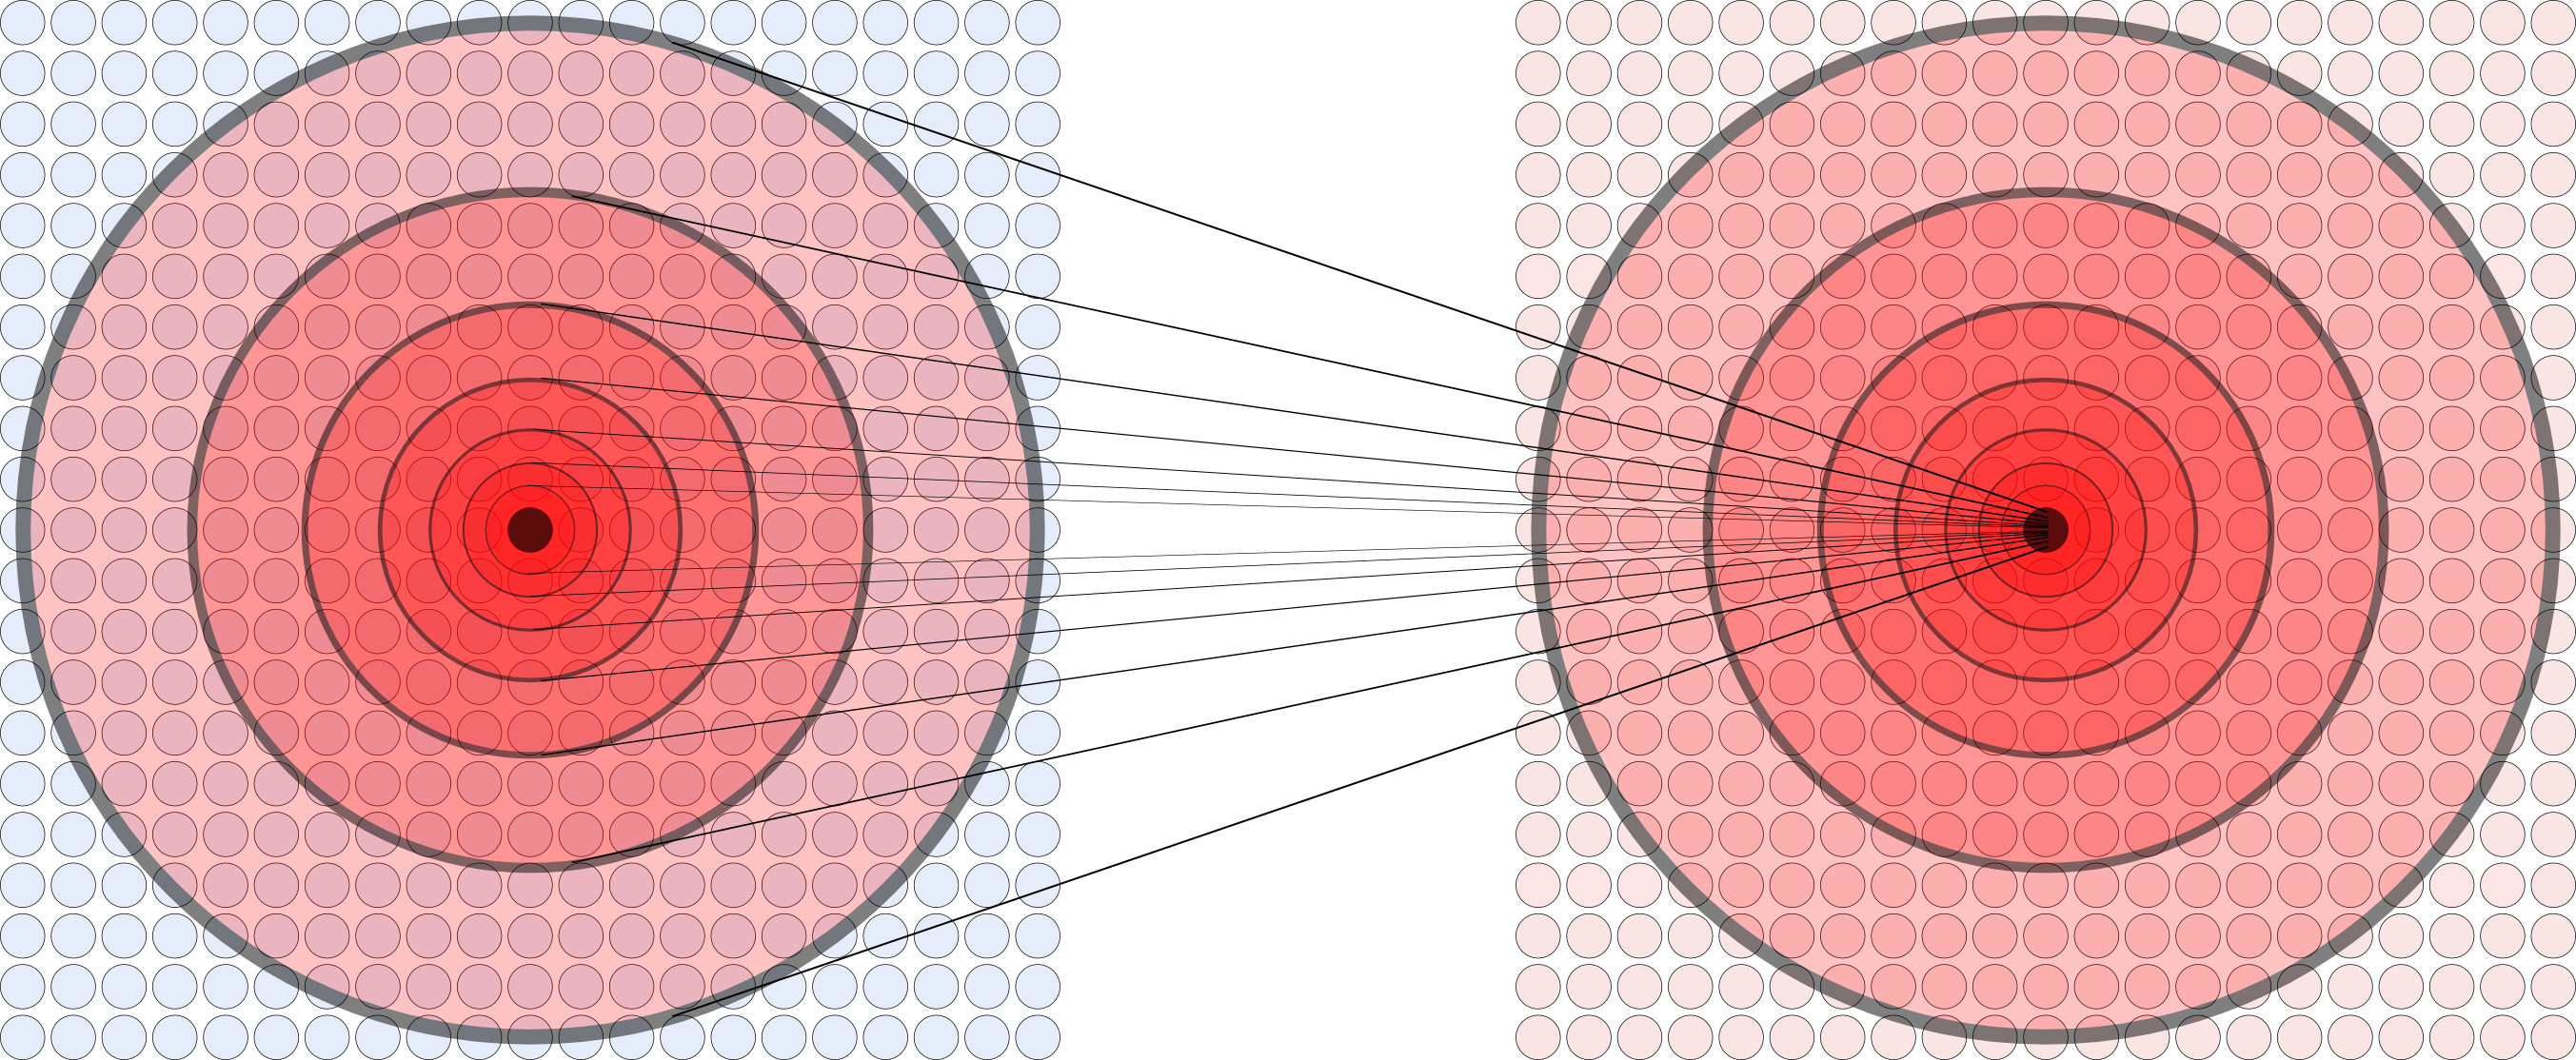
\includegraphics[width=7cm]{fieldsGaussians.png}
  \caption{Neural fields for stability control}
  \label{fig:nf-controller}
\end{figure}


\section{Evolution of Neural Fields}
\subsection{Neural Field Controller Architecture}
The architecture used for the neural field controller uses a structure
similar to that of multilayer perceptrons, i.e. an input layer, a
hidden layer and an output layer. The hidden layer has the properties
so far presented in the neural field model. The input and output
layers are also modeled as a population of neurons but without inner
dynamics. Nonetheless, it is used a kernel for the connection from the
input layer to the hidden layer, as well for the connection from the
hidden layer to the output layer. The input layer is used as a buffer
where sensory inputs are placed before they are processed by the
hidden layer. The output layer is used so that it can be applied some
form of post-processing to the output of the hidden layer without
changing the inner dynamics of the neural field.

\subsection{Evolutionary Algorithm Structure and Parameters}
For the evolution process it is used a simple evolutionary algorithm
as shown in the preliminaries, with random elimination of individuals
inversely proportional with its fitness.

% , but with the addition of niching in the
% for of Deterministic Crowding (see \cite{referencia-dc}), in order to
% promote additional diversity and to prevent premature convergence.

The evolution parameters are the connection kernels between the input
layer and the hidden layer, and between the hidden layer and the
output layer. The recurrent connections of the hidden layer with
itself are left fixed, in the form of a wizard hat function.

The connection kernels are considered isotropic and homogeneous along
the field, so that they can be described as symmetric one-dimensional
arrays of values. 

\subsection{Genotypic Representation and Evolution Operators}
Each connection kernel can be represented as an array of $N$ values
from $w(0)$ to $w(p)$ with homogeneous spacing, using their
symmetry. This way, for an equal boundary radius for all the kernels,
and a 2-layered architecture, there are $2N$ real values in the
genotype. As can be seen, the number of evolution parameters does not
have a direct relation with the simulation size of the neural fields
(the number of discrete points used), in contradistinction with
recurrent neural networks, where the number of parameters depends on
the number $n$ of neurons with a polynomial order
$O(n^2)$. Nonetheless, here is taken a more general approach and the
boundary radius is set equal to $n$, so that there are $O(n)$
parameters.

The evolution operations used in both steps are:
\begin{itemize}
\item Parametric mutation of input array: Gaussian modification of
  real codified array values, which varies the connection kernel
  between input layer and processing layer.
\item Parametric mutation of recurrence array: Gaussian modification
  of real codified array values, which varies the recurrent connection
  kernel of the processing layer.
\item Selection: Calculates population fitness, selects with elitism
  and culling (5\% of both) couples of parents for generating new
  off-springs, calculates the fitness function for both off-springs.
\end{itemize}

The mutation operators implemented apply the sum operator defined in
eq. \ref{eq:eq-leb-opers} but there was not implemented a crossover
operator that used the scalar operator as it was not deemed necessary,
but can be easily implemented for another application if it is
considered useful.

\subsection{Fitness Function}
The fitness function is selected in such a way that the stability
controller mainly has the goal to reduce inclination. It was tuned
experimentally to attain a convergence velocity suitable for the
experiment. This has in mind a notion of sequential evolution of,
first, the capability to attain equilibrium, and later, the capability
to perturb the equilibrium controller in such a way that a planned
trajectory can be followed or a reference can be tracked. Here we are
interested only on the stability problem.

The fitness function for the stability controller is:

\begin{equation}
  F_1=100-\frac{100}{(\pi^4+2)T_{total}}\sum_t{\left(\theta(t) ^4+\frac{|x(t)|}{10}\right)}
\end{equation}

This fitness function aims to minimize the orientation error, but also
has as a minor second goal to minimize the total horizontal
displacement.

While the above expression was used to get the fitness value, the
actual fitness function includes running a simulation instance of the
control problem with a neural field controller grown from the two
kernel arrays.

\section{Experimental Framework}
The model used consists of an approach to biped walking based on a
inverted pendulum (car-and-pole) system in which the pendulum
equilibrium is looked for. Nonetheless, supposing that the pendulum
mass represents the body center of mass, it is proposed that is
reasonable to expect a system with its sole function being to
stabilize the body. This way, the navigation system has as purpose to
carefully perturb the first controller in such a way that the
stabilizing controller moves the car to the desired position. Here we
are particularly interested only on the stability problem and
controller.

\subsection{Dynamic Model}
The dynamic model used, in mathematical terms, is expressed in the two
equations:

\begin{align}
  \ddot{x}&=\frac{F+ml\dot{\theta}^2\sin\theta-mg\cos\theta\sin\theta}{M+m\sin^2\theta}\\
  \ddot{\theta}&=\frac{(M+m)g\sin\theta-F\cos\theta-ml\dot{\theta}^2\sin\theta\cos\theta}{l(M+m\sin^2\theta)}+\frac{\tau}{ml^2}
\end{align}

This model consists of four state variables and a high non-linearity
as it departs from equilibrium points. It is worth noting that the
wanted equilibrium point is in fact unstable.

The output from the stability controller maps to the lateral force
$F$. The angular actuator with value $\tau$ is left to a value of
zero, to allow the plant to behave according to its natural dynamics
on the angular coordinate.

\section{A RNN Approach for Comparison}
The proposed architecture for the recurrent neural network controller
has two expert recurrent networks, whose interaction will achieve
positioning and equilibrium as well.

There has been applied a preprocessing stage previous to the input
neurons, so that the actual values are not used and instead the inputs
are mapped to 3 fuzzy sets. In this way, the stability controller only
has 3 inputs, while the positioning controller has 6, corresponding to
the same 3 inputs previously described and another 3 due to the fuzzy
mapping of the error signal. All neurons are interconnected and the
first one of them is selected as output without loss of
generality. 
% The neural network topology for the first controller
%(stability) is shown in the figure \ref{fig:rnn-arch}.

% \begin{figure}[t]
%   \centering
%   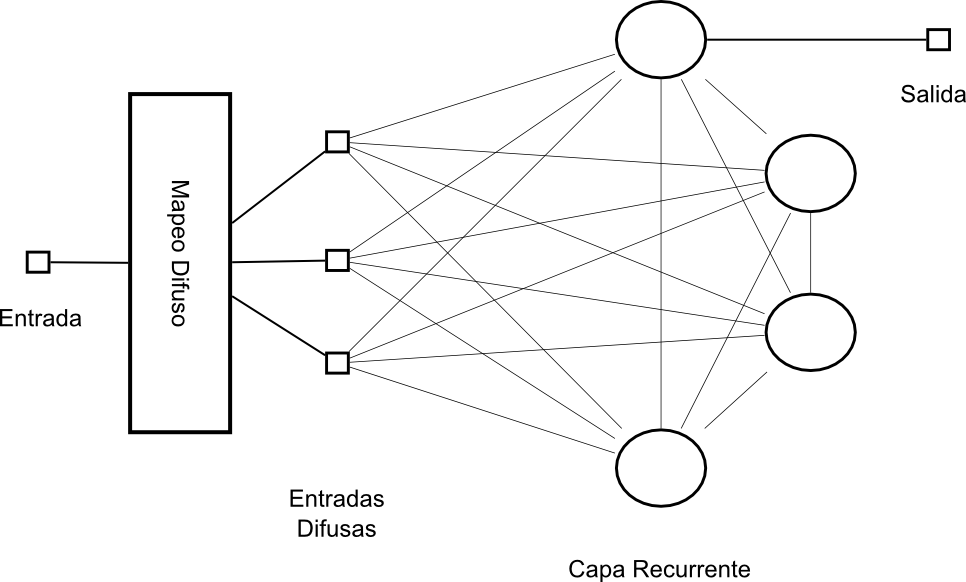
\includegraphics[width=7cm]{rnn.png}
%   \caption{Neural net for stability control including fuzzy mapping}
%   \label{rnn-arch}
% \end{figure}

\subsection{Evolutionary Algorithm Structure for the RNN Controller}
It is expected, based on the approach of artificial life to
evolutionary robotics (Nolfi and Floreano), that the sequential and
cooperative evolution of elements with biological similarity leads to
an specialization in the process of stabilization and positioning
(despite the antagonistic individual goals of each controller because
of the interest of the positioning controller to maximize also the
global performance).

As said, the two steps are executed sequentially, taking the best
individual of the first step to collaborate with the individual
evolved in the second step.

Aiming to obtain a fixed length representation and limit the problem
dimensionality, it is used a model of order $Q$ totally connected. Any
network with an order equal or lesser and with total or partial
connections can be represented by the proposed model, by the addition
of activating/deactivating elements for neurons and
connections. Therefore, individual are codified as:

\begin{itemize}
\item A bit sequence representing a serialization of an activation
  matrix $A_a$ of dimension $Q$-by-$Q$ which activates/deactivates a
  recurrent connection.
\item A sequence of real numbers representing a serialization of
  matrices $W_a$ and $W_b$, of dimension $Q$-by-$Q$ and $Q$-by-$(m+1)$
  respectively.
\end{itemize}

The $C$ matrix is not evolved because it is chosen arbitrarily only
one output (the first neuron).

The evolution operations used in both steps are:
\begin{itemize}
\item Parametric mutation of inputs: Gaussian modification of real
  codified matrix weights, which varies connection weights of inputs.
\item Parametric mutation of recurrences: Gaussian modification of
  real codified matrix weights, which varies connection weights of
  recurrences.
\item Selection: Calculates population fitness, selects with elitism
  and culling (5\% of both) couples of parents for generating new
  off-springs, calculates the fitness function for both off-springs.
\end{itemize}

The fitness functions used are the same presented for the neural field
controller.

\section{Experimental Results}
\subsection*{Experimentation Details}
The sampling time used was $0.025$s (for neural networks, neural
fields, and visualization) and $10$ s tests were performed.

The differential equation system was solved by a fixed-step numerical
method, 4th Order Runge-Kutta. The iteration step selected was also
$h=0.025s$ for each test.

Here are shown the results obtained for:
\begin{itemize}
\item The evolved RNN controller
\item A (non-evolved) neural field controller only with an input
  layer. It uses directly the input field activation to control the
  system (that is, it actually does omits the processing field to
  perform the control).
\item The non-evolved neural field controller. An appropriate
  selection of parameters is applied (made taking into account only
  the self-stability of the neural fields and the time constants of
  the plant). It behaves roughly as a proportional state space
  controller.
\item The evolved neural field controller (also with an appropriate
  selection of parameters).
\end{itemize}

For all the simulations, the initial angular position was
$\theta=\pi/6$, the number of discrete positions used in the
simulation of the neural field was $21$, and the angular position
$\theta$ was encoded into the input field with value $1$ while the
angular velocity $\omega$ was coded with value $k_\omega=0.5$. The
neural field time constant was taken with value $\tau=1/10$s. The
filtering (wizard hat) kernel on the actuator had values $k=1$,
$\delta=2$ and $H_0=0$. Also, the maximum control signal energy was
equal for all the simulations (and architectures) presented.

For the non-evolved controller, it were used also wizard hat kernels
as defined in eq. \ref{eq:wizard-hat}. The input kernel had values
$k=2$, $\delta=2$ and $H_0=0.1$. The processing kernel had values
$k=0.3$, $\delta=2$ and $H_0=0.1$. Those values were derived mostly by
trial-and-error.

For the evolved controller, there were used parametrized kernels feed
by the kernel arrays on the genome of the evolutionary algorithm. The
Gaussian mutation operators were initialized with a standard deviation
of 0.3. Its application rate is evolved itself by the evolutionary
algorithm used, which adjusts the operators rates on-line (Hybrid
Adaptive Evolutionary Algorithm).

\subsection*{Results}
\paragraph{RNN Controller}
The first experiment is performed using the recurrent neural network
controller without evolution. Results are presented in the figure
\ref{inestabilidad}. The figure shows the natural dynamics of the
system when the controller is randomly parametrized. It can be
perceived the need for the parametrization made by the evolutionary
algorithm on the recurrent neural network controller, since the
inverted pendulum is an unstable system around the origin, and a
random controller can not stabilize it. Red dots represent the pole
mass location and blue dots represent the cart position.

\begin{figure}[h]
  \centering
  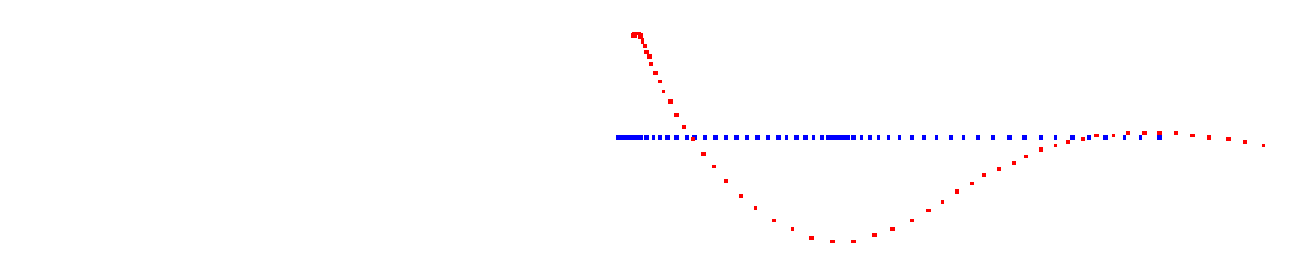
\includegraphics[width=7cm]{chp2-ijcnn-inestabilidadG}
  \\
  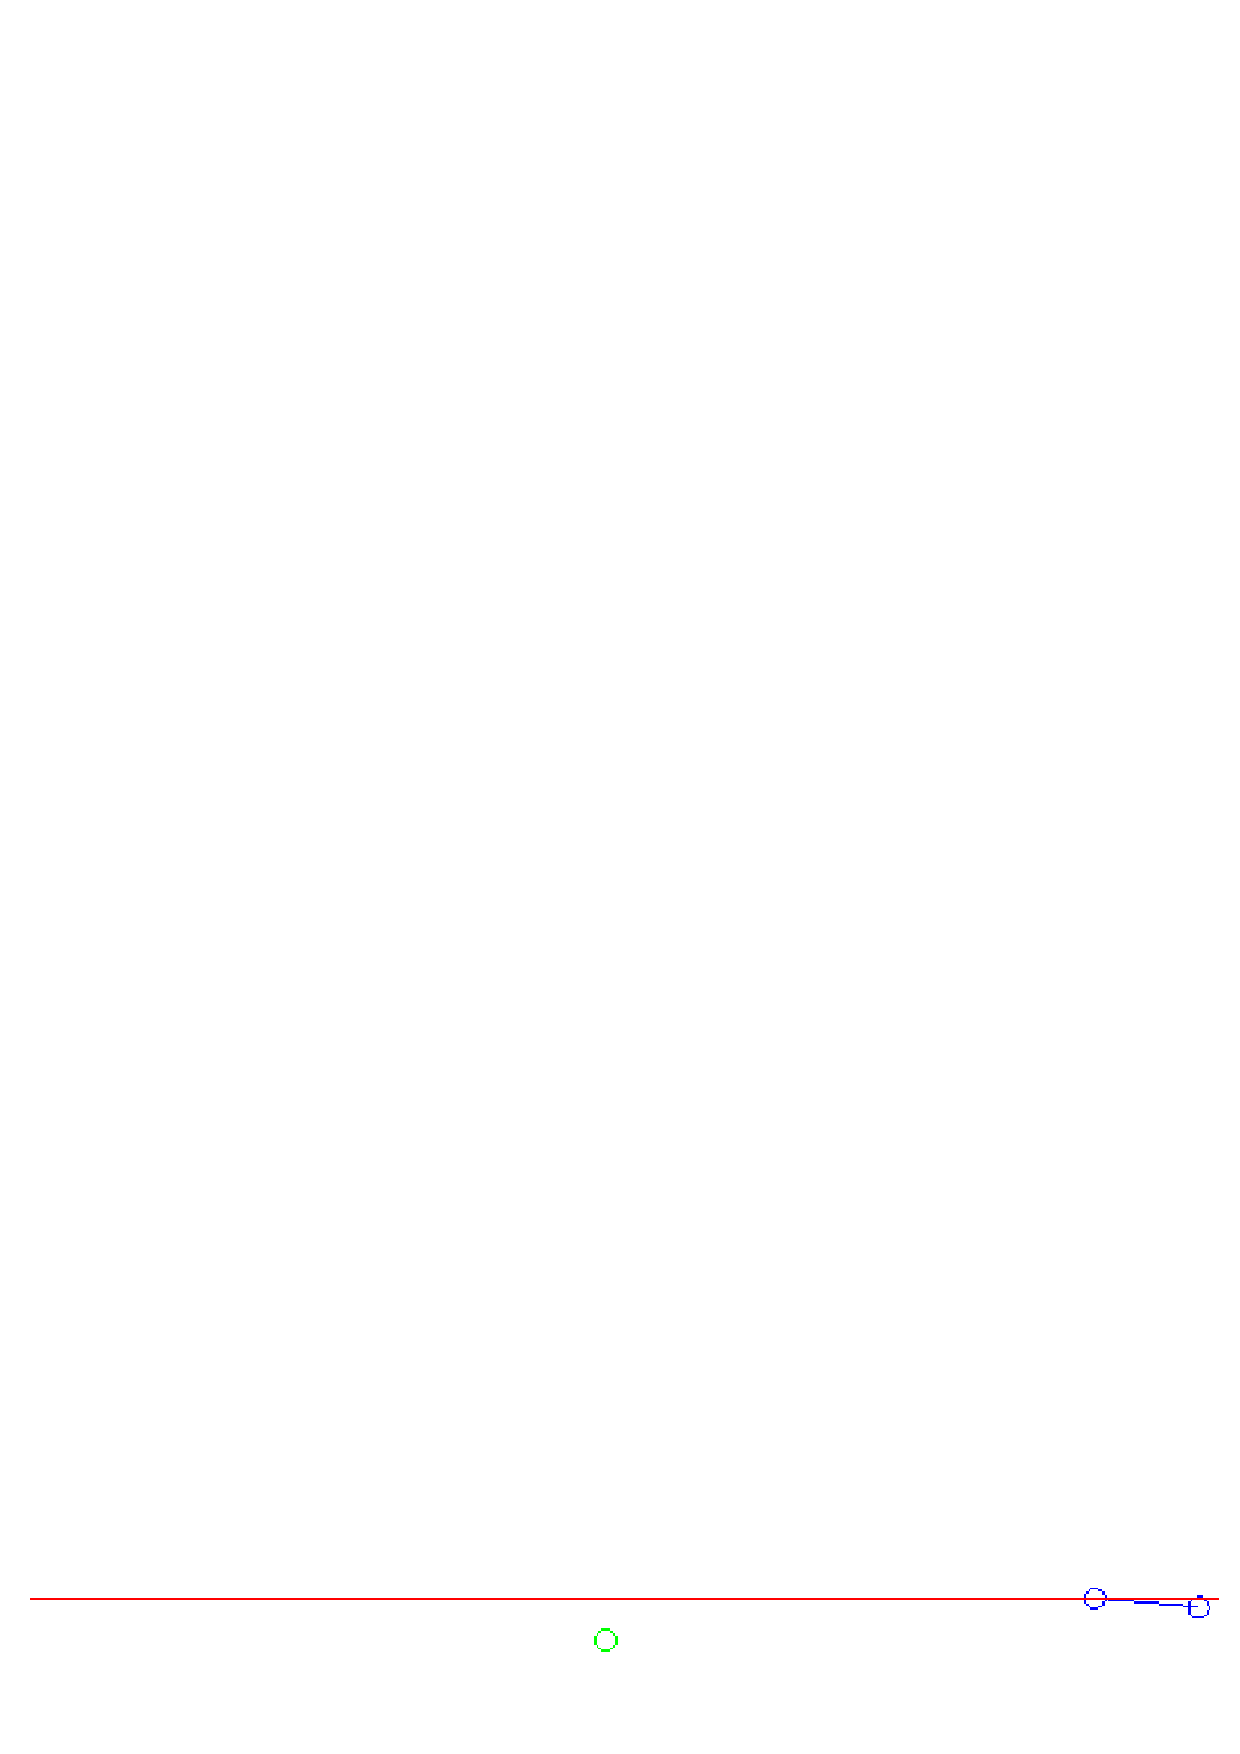
\includegraphics[width=7cm]{chp2-ijcnn-inestabilidadC}
  \caption{System dynamics with an untrained RNN controller. The first
    figure shows the pendulum trace, and the second shows the pendulum
    at $t=3.5$s.}
  \label{inestabilidad}
\end{figure}

The second experiment shows the behavior of the inverted pendulum once
the RNN controller has been evolved. Results are presented in figure
\ref{rnnSimulation}. The adaptation made by the evolutionary
algorithm, as is evident, has an important positive effect on the
controller.

\begin{figure}[h]
  \centering
  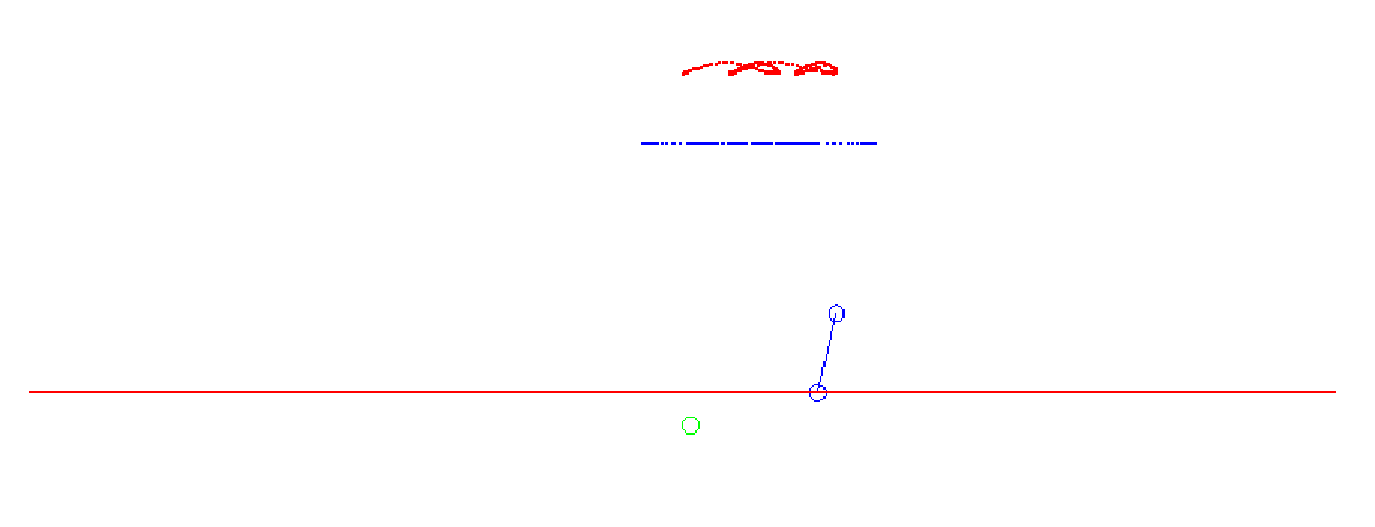
\includegraphics[width=7.5cm]{chp2-ijcnn-rnnSimulation}
  \caption{System dynamics with a trained RNN controller. The first
    figure shows the pendulum trace and the second the pendulum at
    $t=3.5$s.}
  \label{rnnSimulation}
\end{figure}

\paragraph{RNN Controller and Neural Field Controller Comparison}
The next three experiments were performed with: an evolved RNN
controller architecture, a (non-evolved) neural field architecture
using the processing field as output, and a (non-evolved) neural field
architecture using the input field as output (effectively omitting the
processing field in the feedback loop). In the remaining, the neural
architectures will be simply called '(non-evolved) input field
architecture' (the architecture omitting the processing field) and
'processing field architecture' (the non-evolved architecture using
the processing field in the feedback loop).

The qualitative behavior of the non-evolved processing field is shown
in the figure \ref{estabilidad}. It can be seen that, when an initial
angular perturbation is small, the neural field is able to control the
stability without evolution.

\begin{figure}[h]
  \centering
  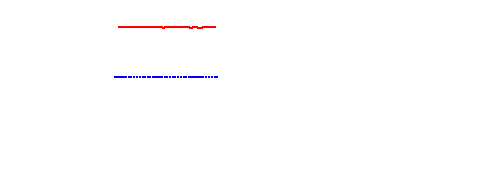
\includegraphics[width=7cm]{estabilidadG.png}
  \\
  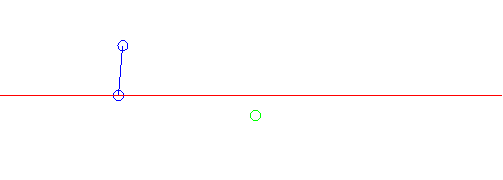
\includegraphics[width=7cm]{estabilidadC.png}
  \caption{System dynamics with a non-trained Neural Field
    Controller.}
  \label{estabilidad}
\end{figure}

Results of these three experiments are presented comparatively in
figure \ref{fig:pendulum-plot}.

\begin{figure}[p]
  \centering
  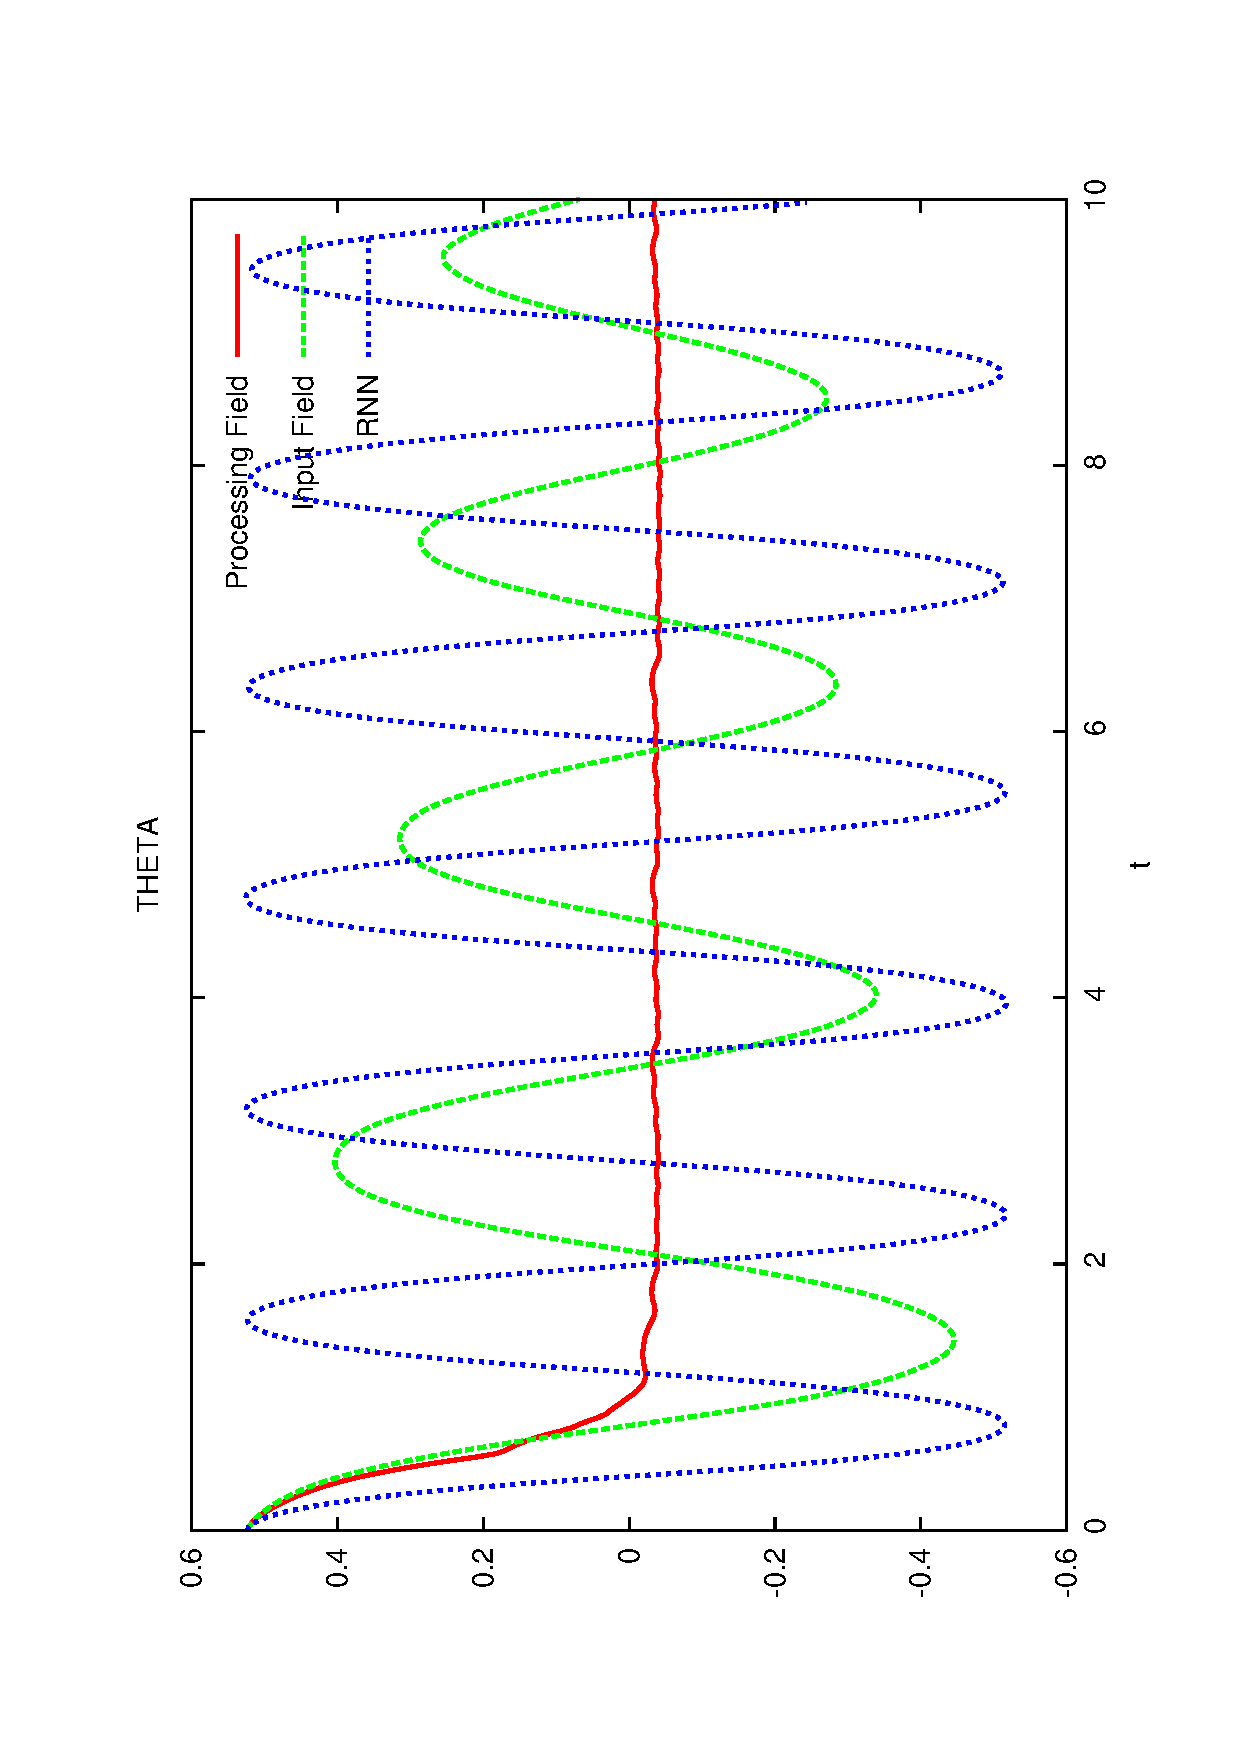
\includegraphics[angle=-90,width=7cm]{chp2-ijcnn-pendulum_thetas}
  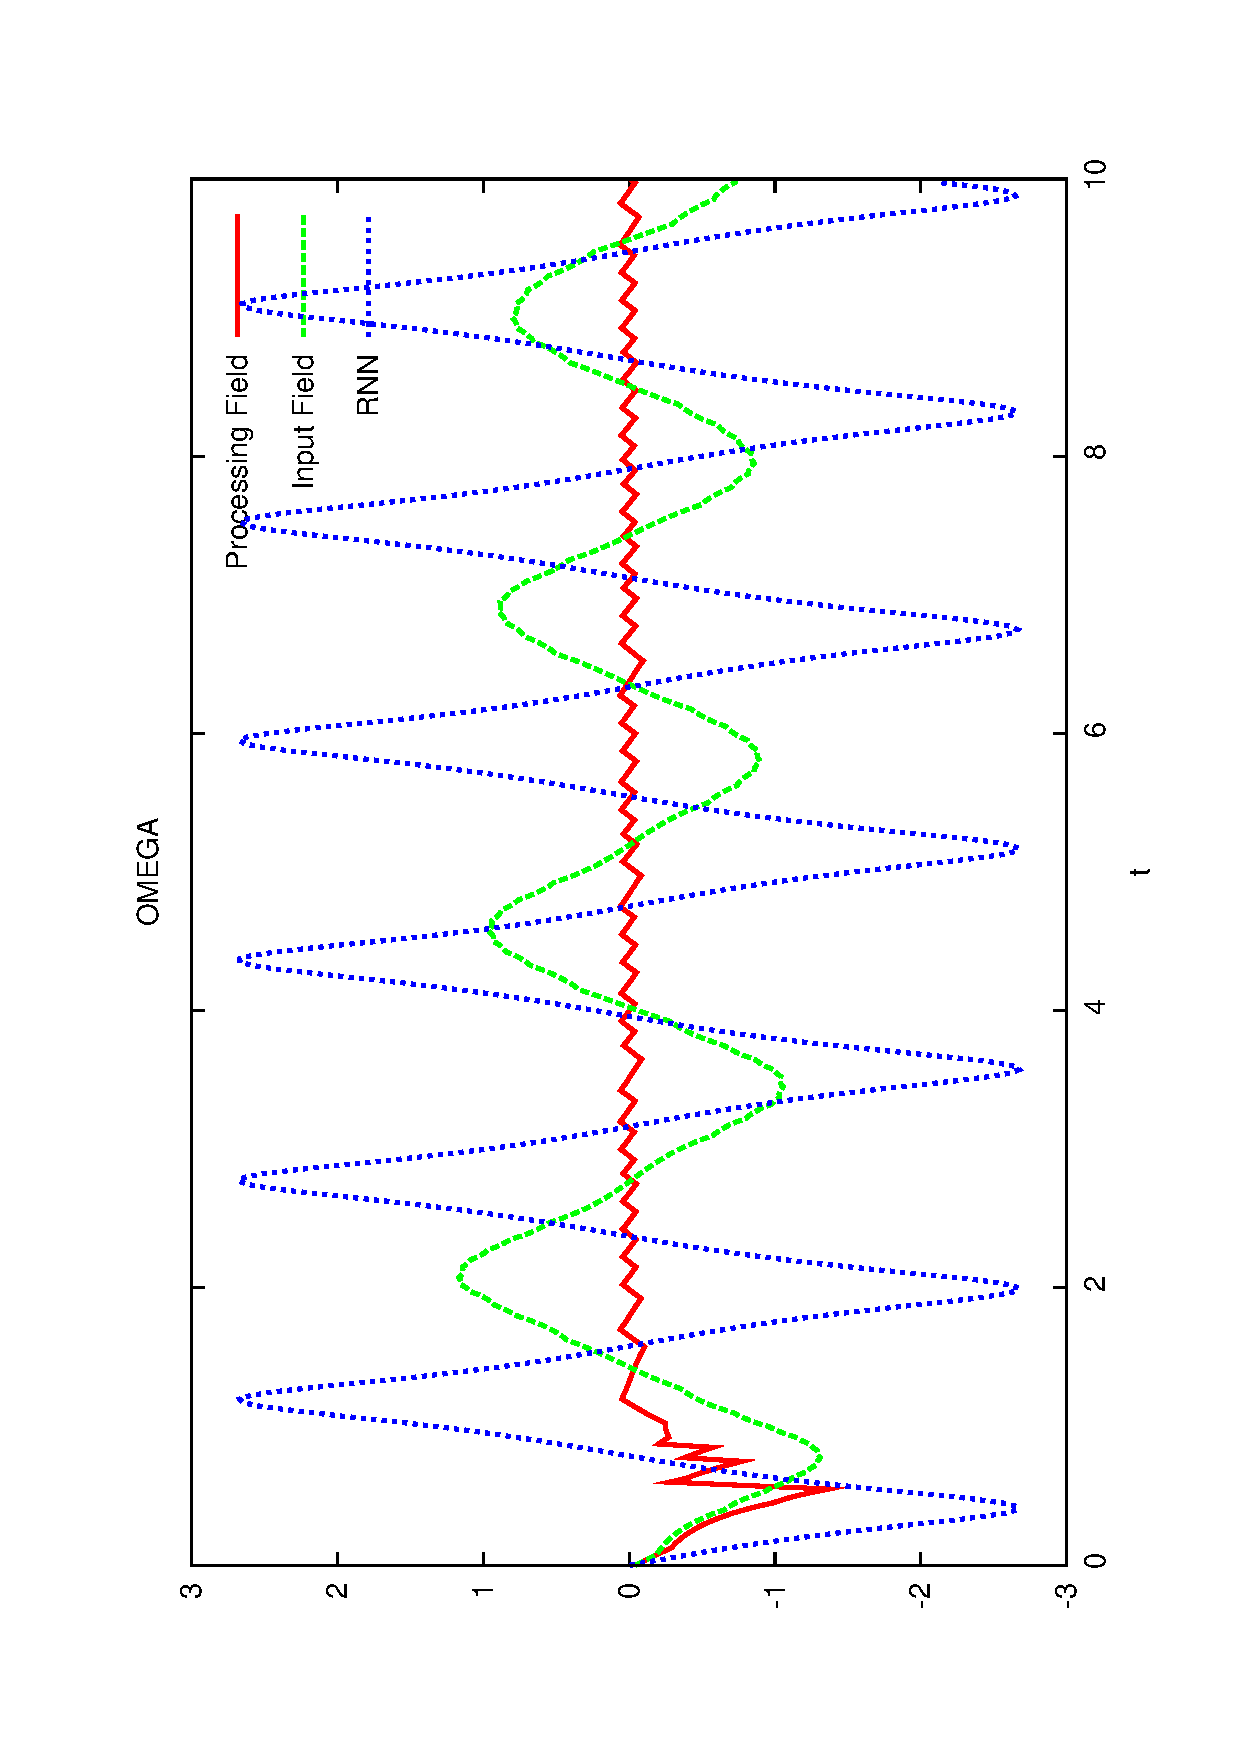
\includegraphics[angle=-90,width=7cm]{chp2-ijcnn-pendulum_omega}
  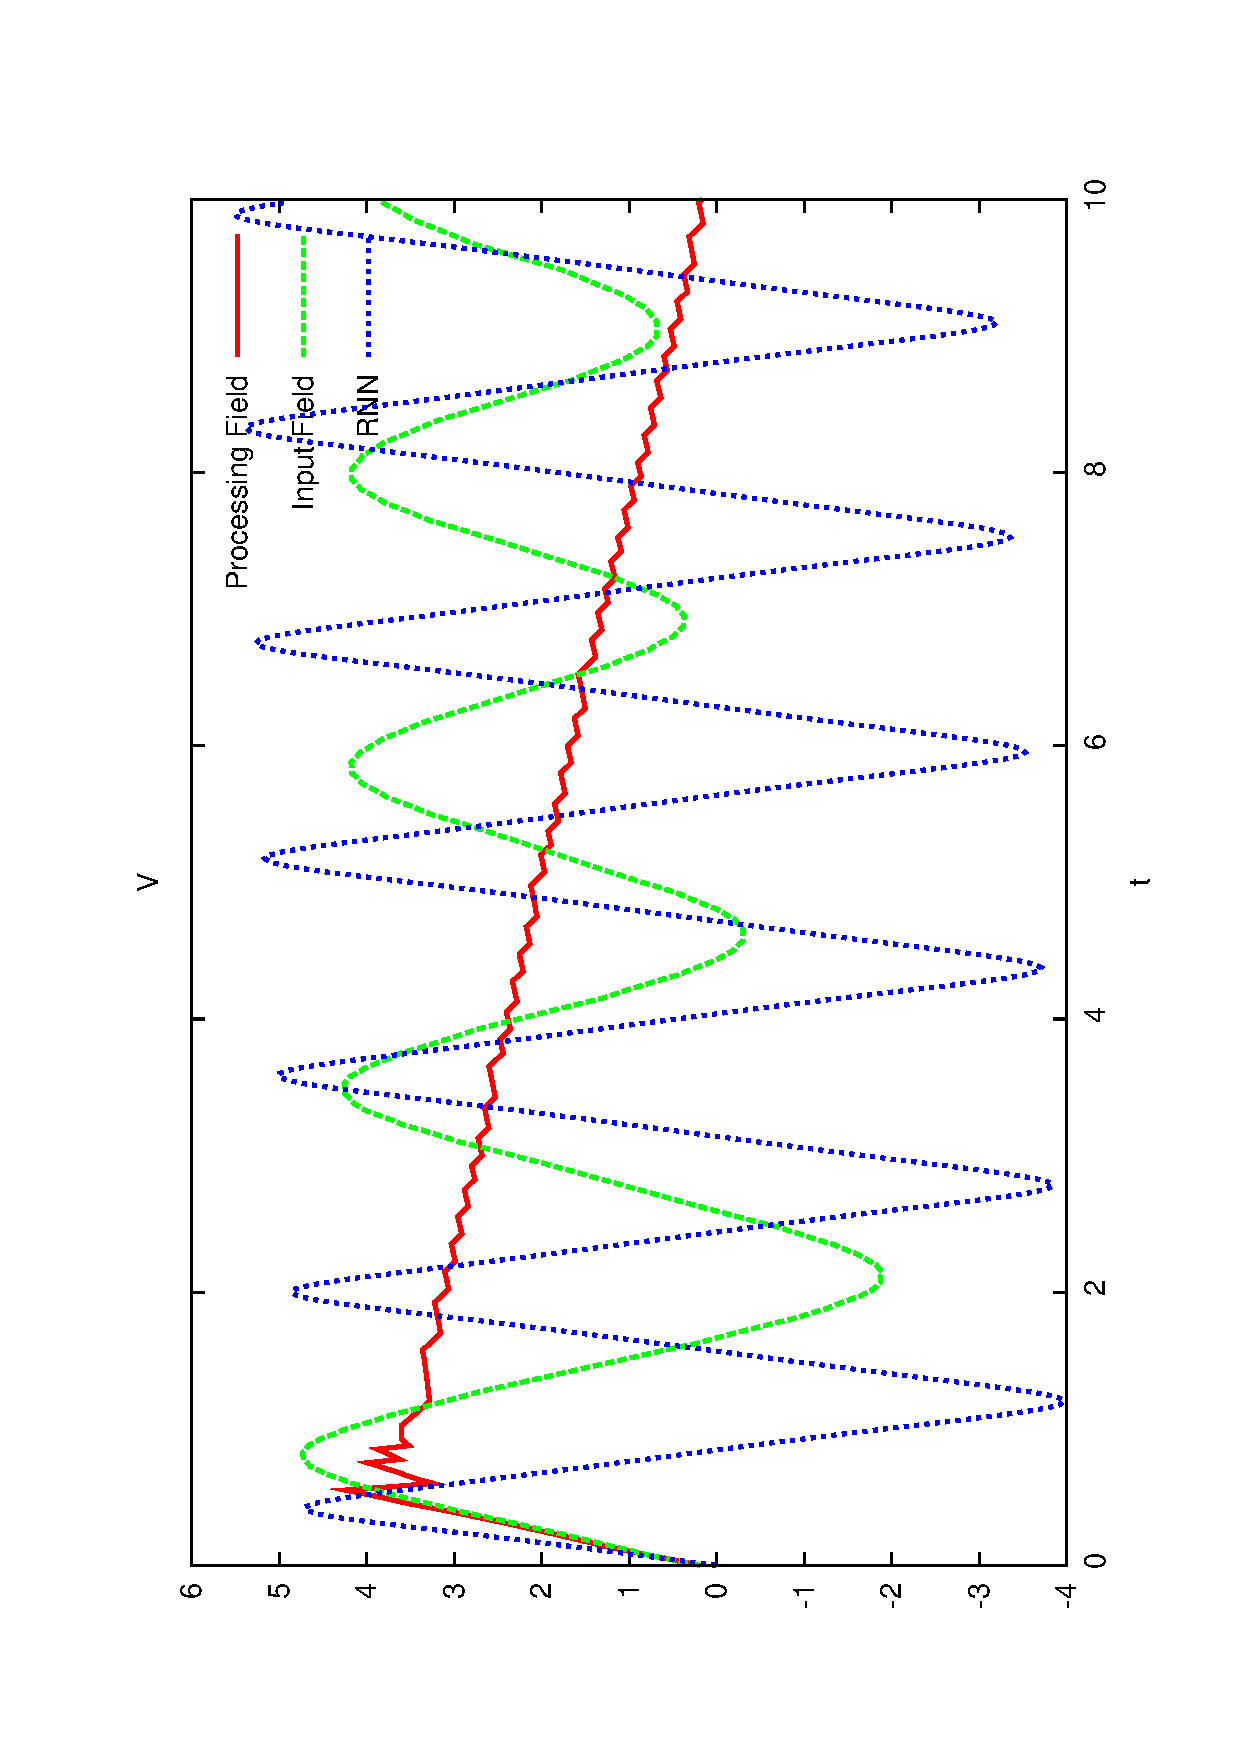
\includegraphics[angle=-90,width=7cm]{chp2-ijcnn-pendulum_v}
  \caption{Pendulum simulations with neural controllers between $t=0$s
    and $t=10$. The three controllers shown are: a RNN controller, an
    input field controller and a processing field controller. In the
    top, the angular position is plotted ($\theta$). In the middle,
    the angular velocity is plotted ($\omega$). In the bottom, the
    linear velocity ($v$) is plotted.}
  \label{fig:pendulum-plot}
\end{figure}

In the upper part of figure \ref{fig:pendulum-plot}, the behavior of
the angular position state variable ($\theta$) is shown. This is the
central variable of the control task, since its minimization would
mean also a minimization of the error signal (viewed from a classical
control theory perspective). Both the recurrent neural network
architecture and the input field architecture (marked as 'input
field') show an oscillating behavior with wide movements around the
reference value ($\theta=0$). Of them, the RNN architecture has the
fastest response, but also the widest oscillations. On the contrary,
the input field architecture shows diminishing oscillations with
increasing time.

On the other hand, the processing field architecture (marked as
'processing field') presents the best performance, staying close to
the reference (with an error $|e_{\theta}|<0.05$) from $t=1.0s$
onwards.

The middle and bottom parts of figure \ref{fig:pendulum-plot} show the
state variables $\omega$ (angular velocity) and $v$ (linear
velocity). The angular velocity plot reinforces the perceptions given
by the angular position plot. It also shows that the responses of the
RNN controller and the input field architecture are smoother than the
response of the processing field architecture.

The linear velocity plot evidences that all controllers deviate
significantly from the initial linear position in the
experiments. This is expected, since the focus was on balancing of the
inverted pendulum, and not on its linear positioning.

While the results shown by both neural field architectures are not
ideal (none of them seems to achieve a zero error signal), their
results are certainly better than expected. This is notable,
considering that the RNN was evolved to solve the task at hand, while
the neural field architectures were manually parametrized, and there
were not applied any adaptation or evolution schemes to their
parametrization.

The recurrent neural network controller is expressive enough to solve
the problem at hand, but the number of parameters to configure (or in
this case to evolve) is of a quadratic order in relation to the number
of nodes (or neurons). This was not a particular problem for the
evolutionary algorithm used, but it can be a limitation if an
adaptation scheme is not applied. Furthermore, the evolutionary
parametrization applied was not able to outperform the manual
parametrization of the neural field architectures.

On the other hand, the neural field controller is a bit more complex
(in its implementation) and its simulation more costly (up to $10$
times slower than the recurrent neural network), but has some notable
advantages. The first one is its ability to self-compensate or,
equivalently, the stability of its natural dynamics, which is attained
after the setup of few parameters. The second one is its suitability
to the problem at hand, being able to solve it with a good
performance. Although there was a need for parameter configuration,
evolution was not required because the number of parameters to setup
is small: basically three parameters of the kernel function and the
resting potential of the field equation --- a number of parameters of
constant order in relation to the number of nodes (discrete elements
on the neural field).


\paragraph{Evolved and Non-Evolved Neural Field Controller Comparison}
A last experiment is performed using the evolved neural field
controller architecture, for the same problem and experimental
setup. Its qualitative behavior is shown in figure
\ref{fig:chp2-evonf-capture}.

\begin{figure}[h]
  \centering
  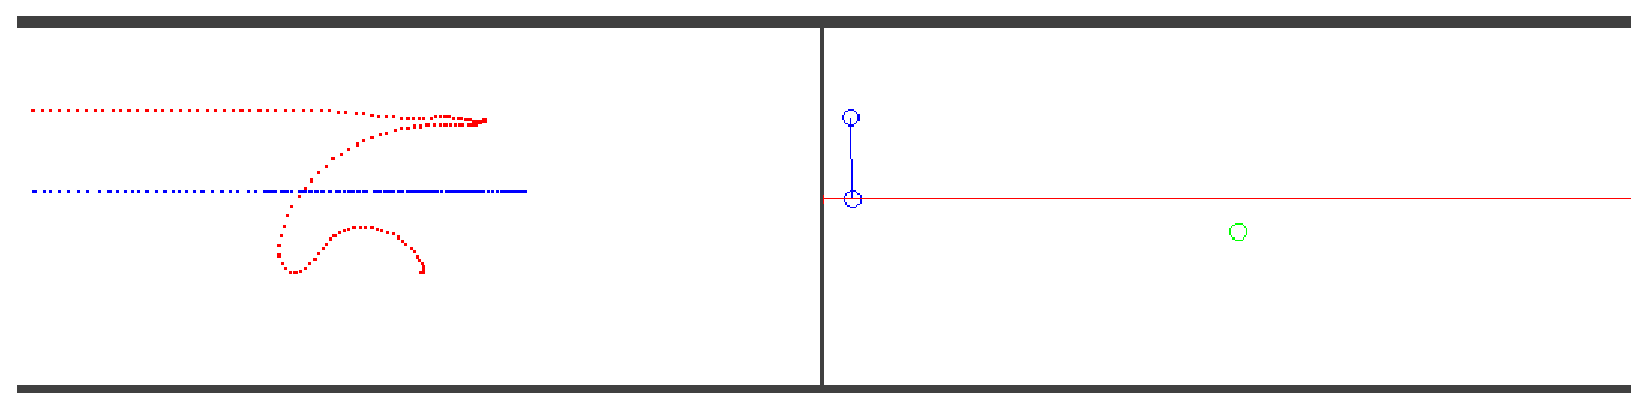
\includegraphics[width=1\textwidth]{chp2-gecco-neuralfield-panel-2}
  \caption{System dynamics with an evolved Neural Field Controller, at
    time $t=4$. Left: trace of the pendulum (cart in blue and pole tip
    in red). Right: snapshot of the animation at time $t$.}
  \label{fig:chp2-evonf-capture}
\end{figure}

The direct controller (non-evolved neural input field architecture)
can by itself attain stability for the initial value $\theta=\pi/6$
but the performance is poor. While not shown, it has problems
stabilizing the pendulum with an initial value of $\theta=\pi/3$ or
higher.

The hand-tuned controller (non-evolved processing field controller) is
able to control the stability without evolution with a better
performance than the presented by the direct controller. It can
stabilize in the 10s time those instances with an initial value of
$\theta=\pi/3$ or higher. Nonetheless, it causes big displacements and
tends to keep a small but persistent orientation error.

Finally, the evolved controller has the best performance of the three,
performs a fast stabilization of the pendulum even with an initial
value of $\theta=\pi$ (worst-case scenario for the initial
orientation), which is shown in figure \ref{fig:pendulum-states}. It is the
only one that stays for long periods of time on the reference
orientation and it causes the least displacements. Despite its
parametrization being carried out by evolution, its strategy can be
understood by looking at processing field activation values, and this
controller seems to apply short burst of switching maximum values.

The three figures \ref{fig:inputs}, \ref{fig:processings} and
\ref{fig:pendulum-states} show the input fields, the processing fields
and the state variables evolution (respectively) for the three
controllers.

\begin{figure} [p]
  \centering
  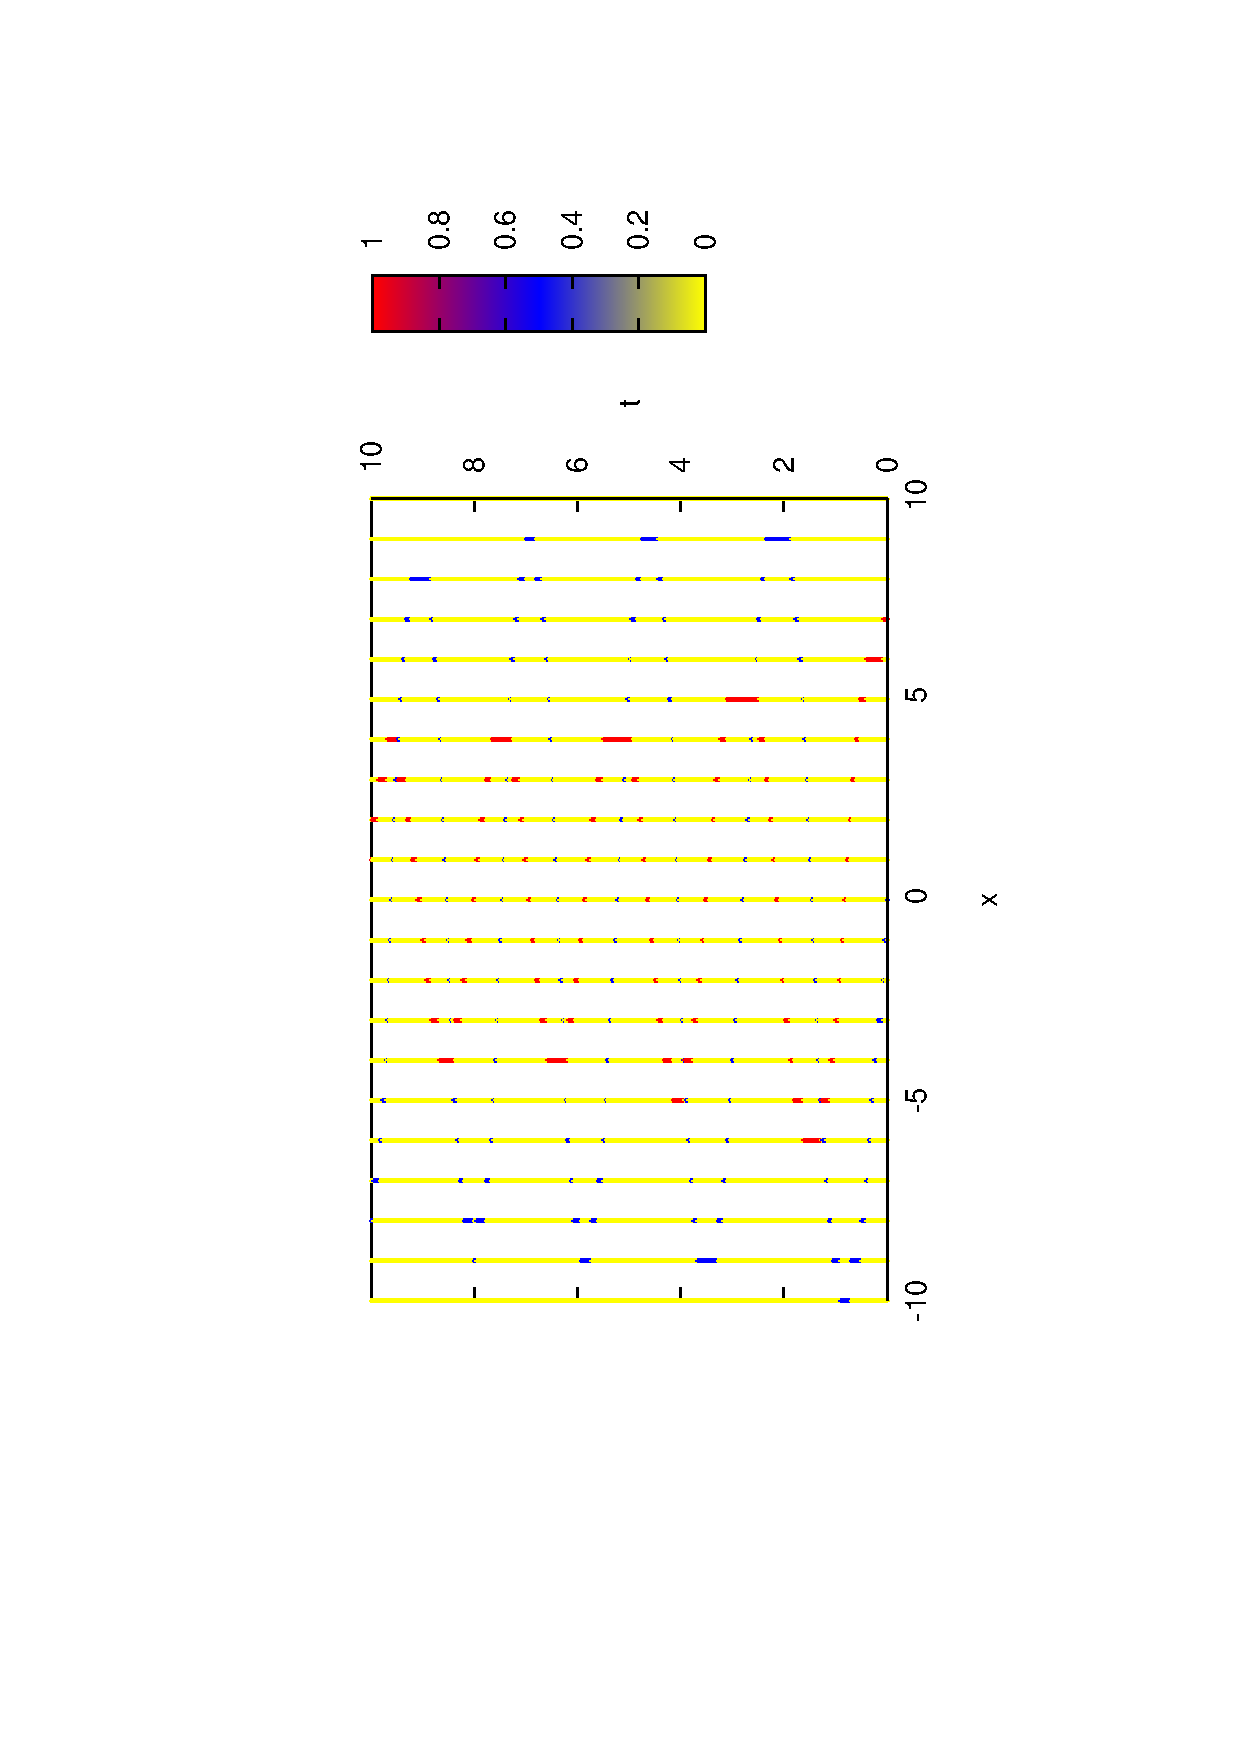
\includegraphics[width=6.5cm,
  angle=-90]{chp2-gecco-inputPopulation_old}
  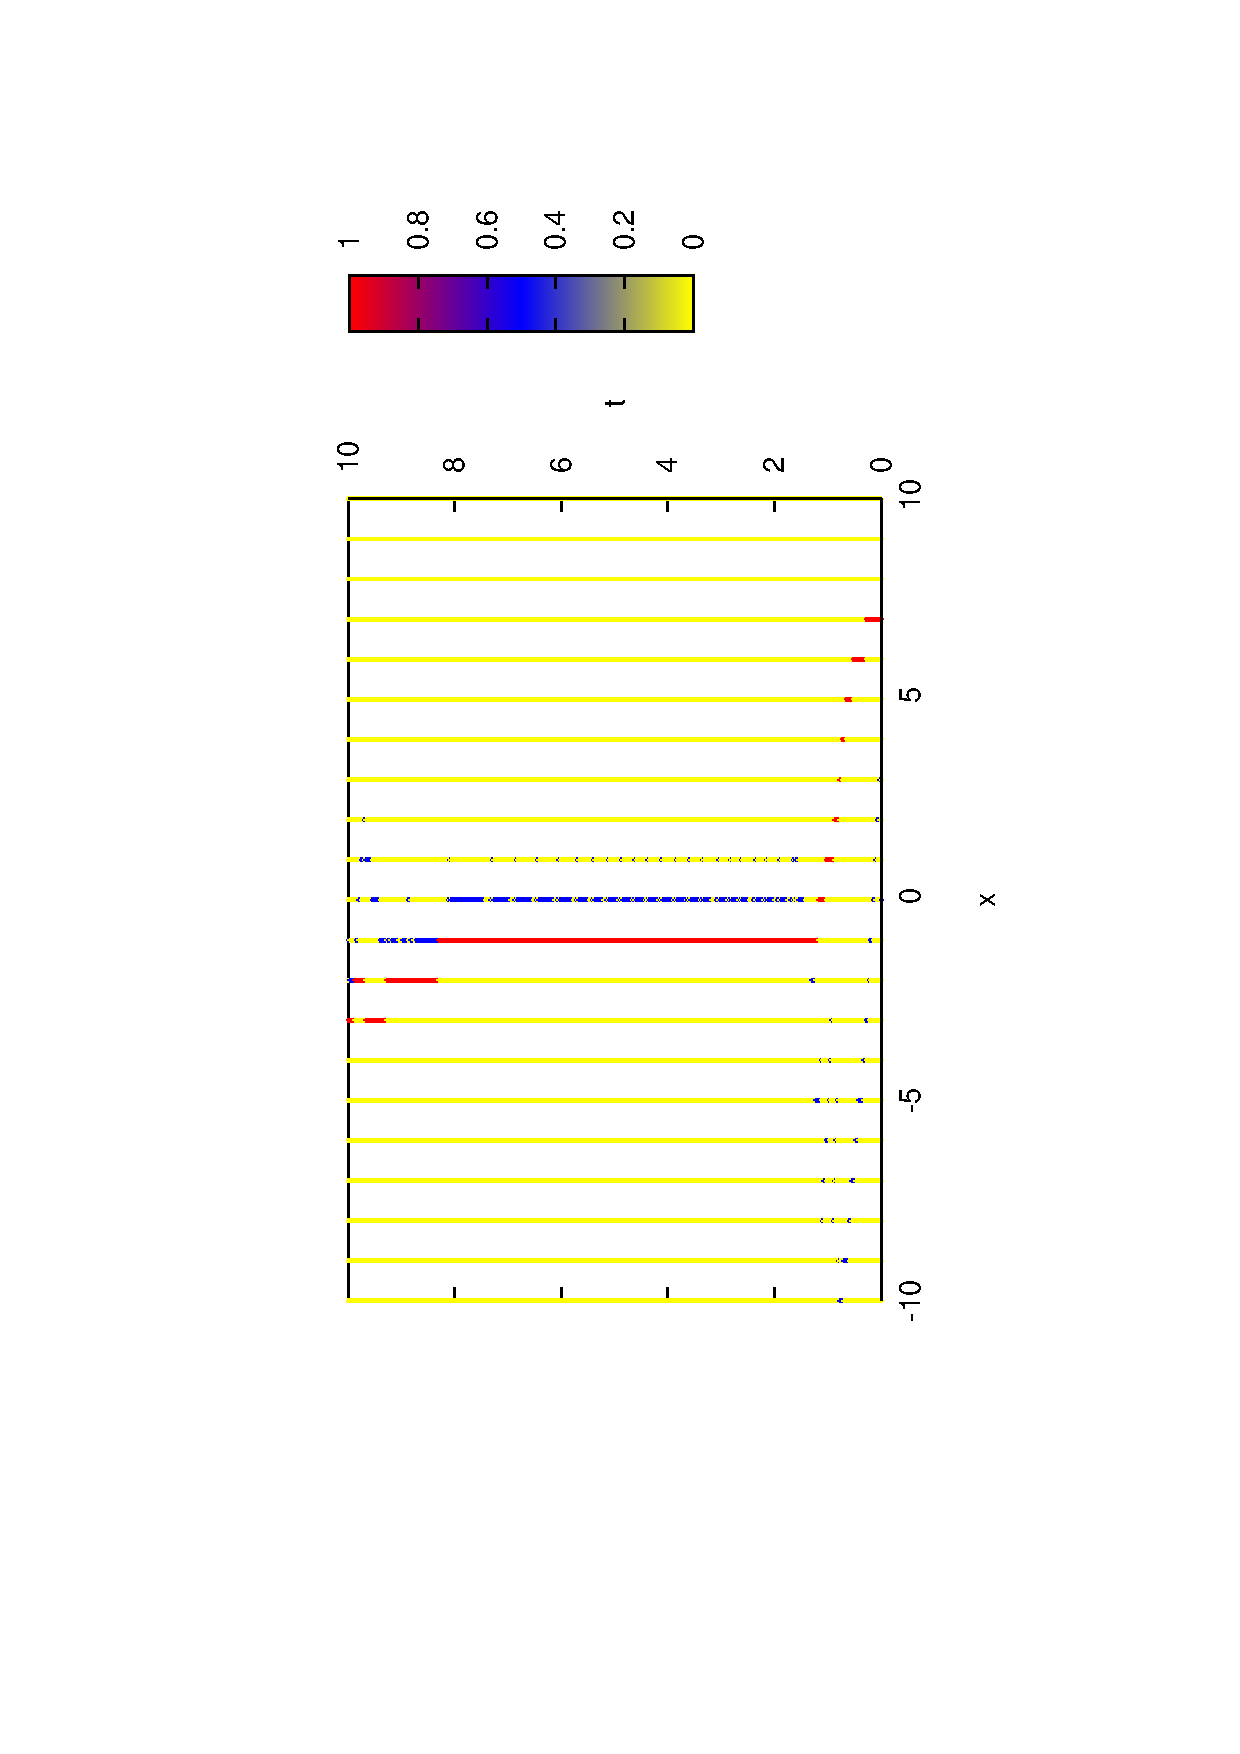
\includegraphics[width=6.5cm, angle=-90]{chp2-gecco-inputPopulation}
  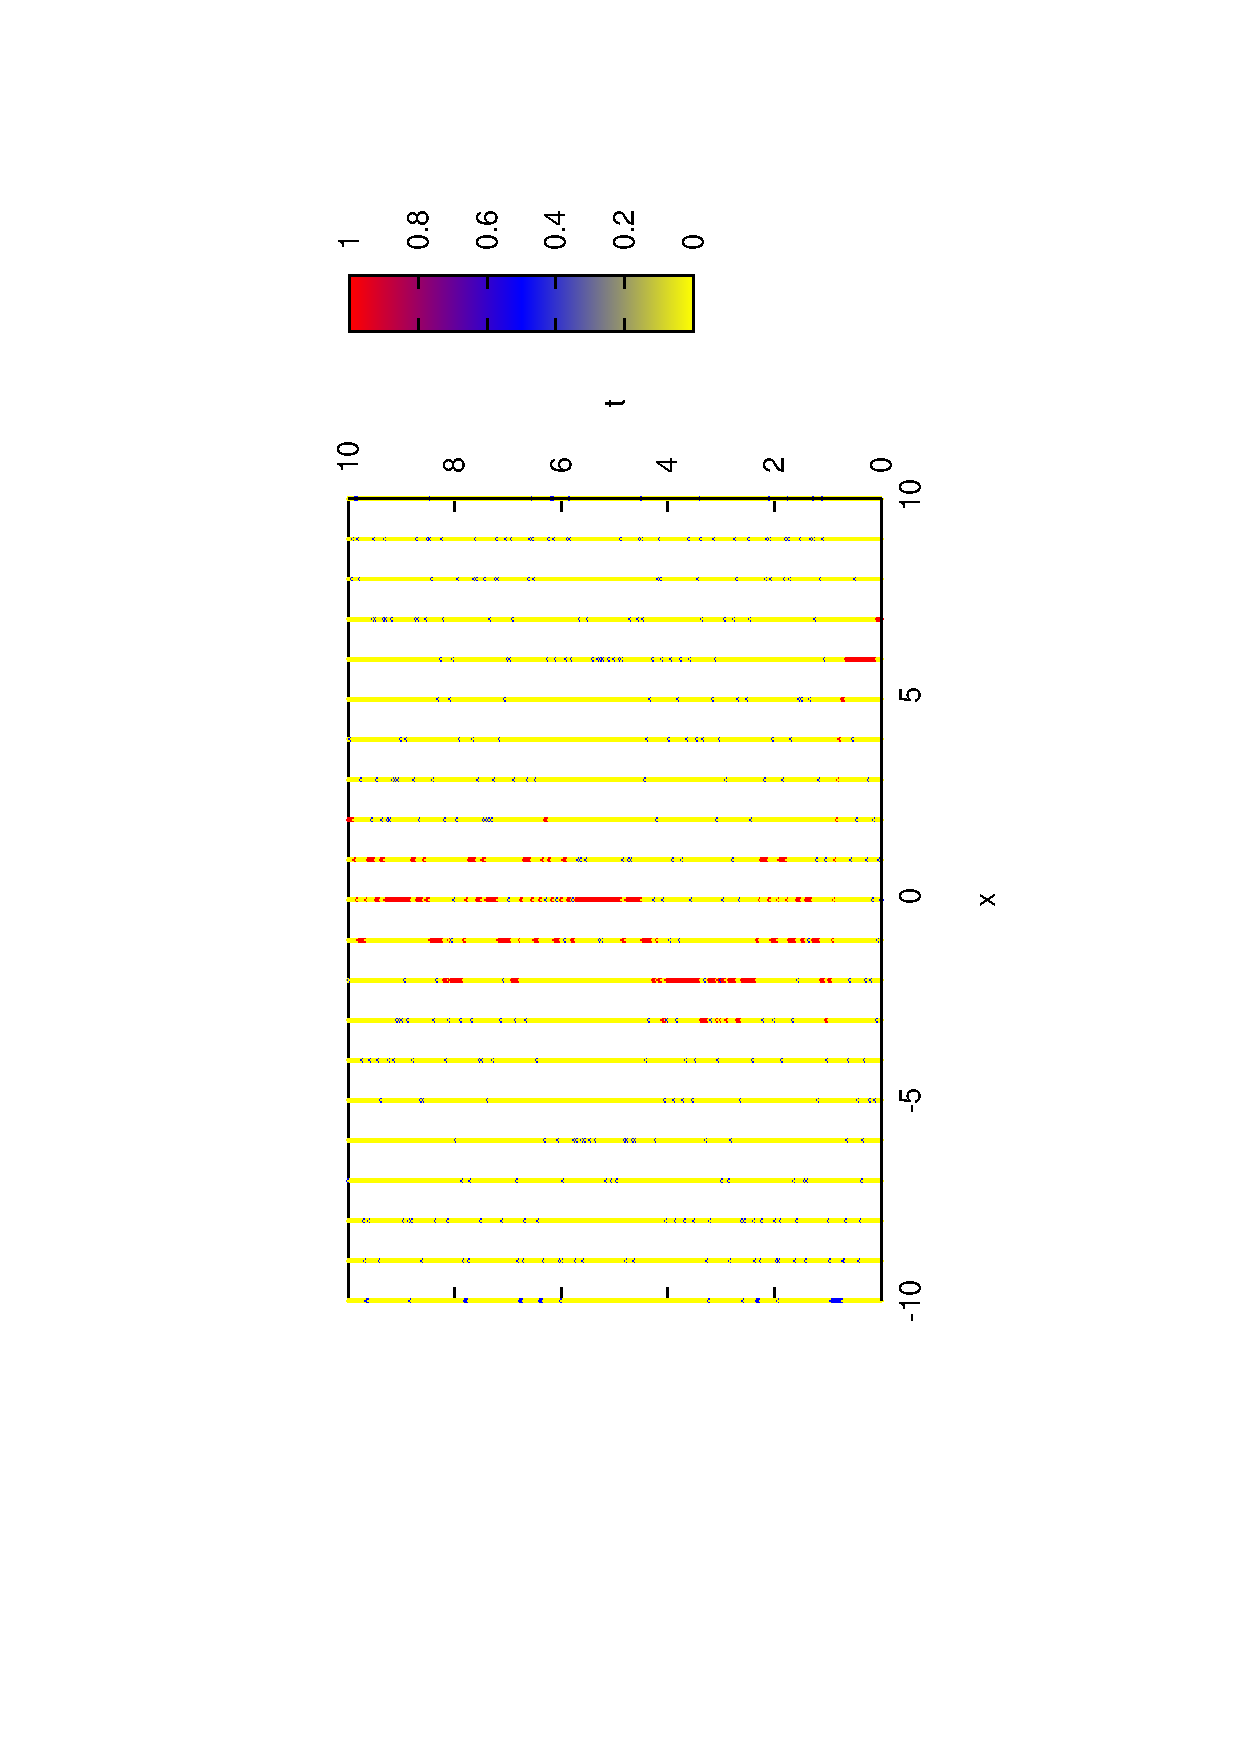
\includegraphics[width=6.5cm,
  angle=-90]{chp2-gecco-inputPopulation_evo}
  \caption{Input layer activation for simulations between $t=0$s and
    $t=10$s with steps $h=1/40$s and positions between $x_{min}=-10$
    and $x_{max}=10$. First: direct (without processing layer)
    controller. Second: non-evolved controller. Third: evolved
    controller.}
  \label{fig:inputs}
\end{figure}

In the figure \ref{fig:processings}, of processing layer activations,
the horizontal ($x$) axis represents the position of each element on
the one-dimensional processing layer population, and the oblique axis
($t$) represents the time elapsed. The presence of the processing
field in the feedback loop appears to act as an integrator-like
control element. On the contrary, the sole utilization of the input
field to spatially code the inputs appears to act as a proportional
control element, causing the highly oscillating behavior in the input
field architecture. Consequently, the nonlinear coupling between both
actions, integral-like and proportional, seems to produce the behavior
presented by the processing field architecture. Furthermore, the
activation of the evolved neural field is quite chaotic, but shows a
preferential activation on the extremal points, which could be
interpreted as a preference for application of maximum control values
(may be as an approximation of a bang-bang controller).

% \begin{figure}[p]
%   \centering
%   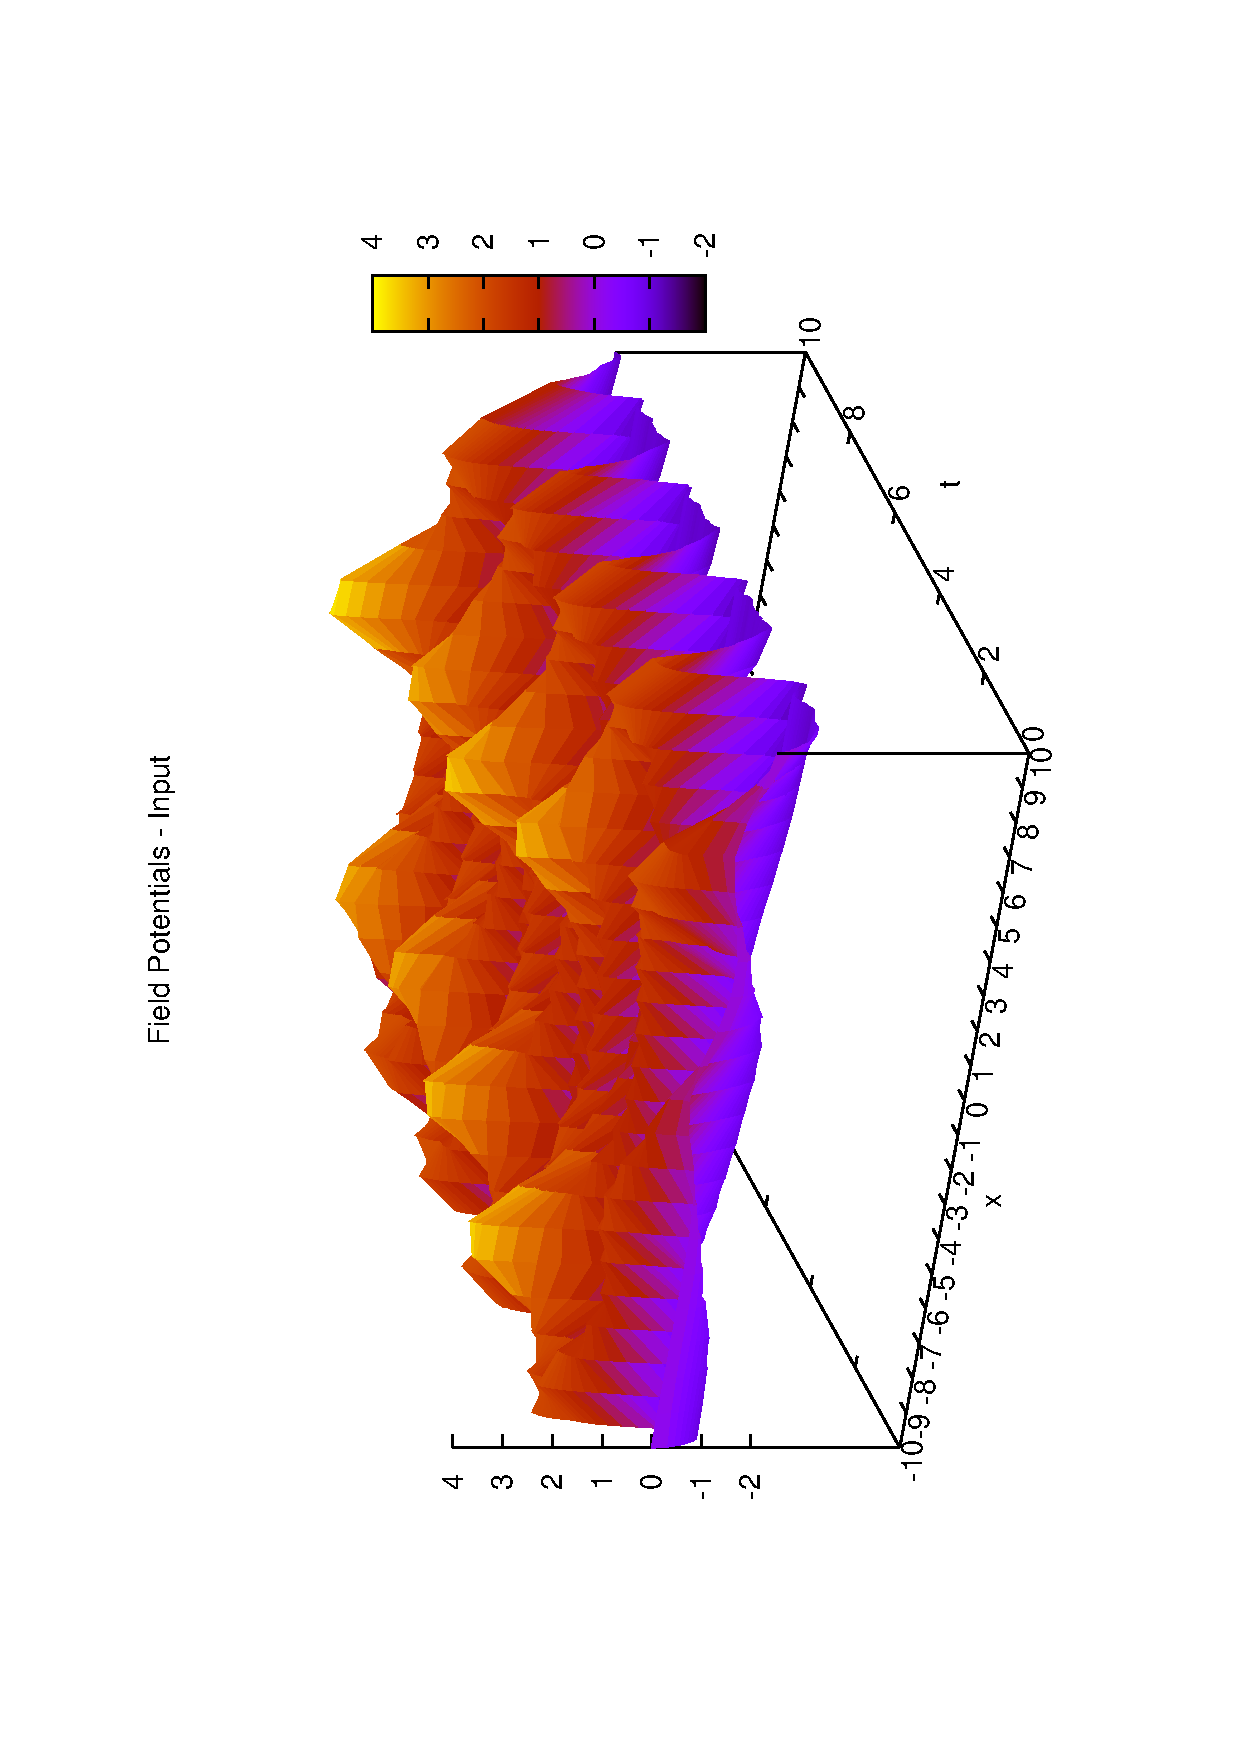
\includegraphics[angle=-90,width=7cm]{chp2-ijcnn-fieldPopulation_ijcnn_old}
%   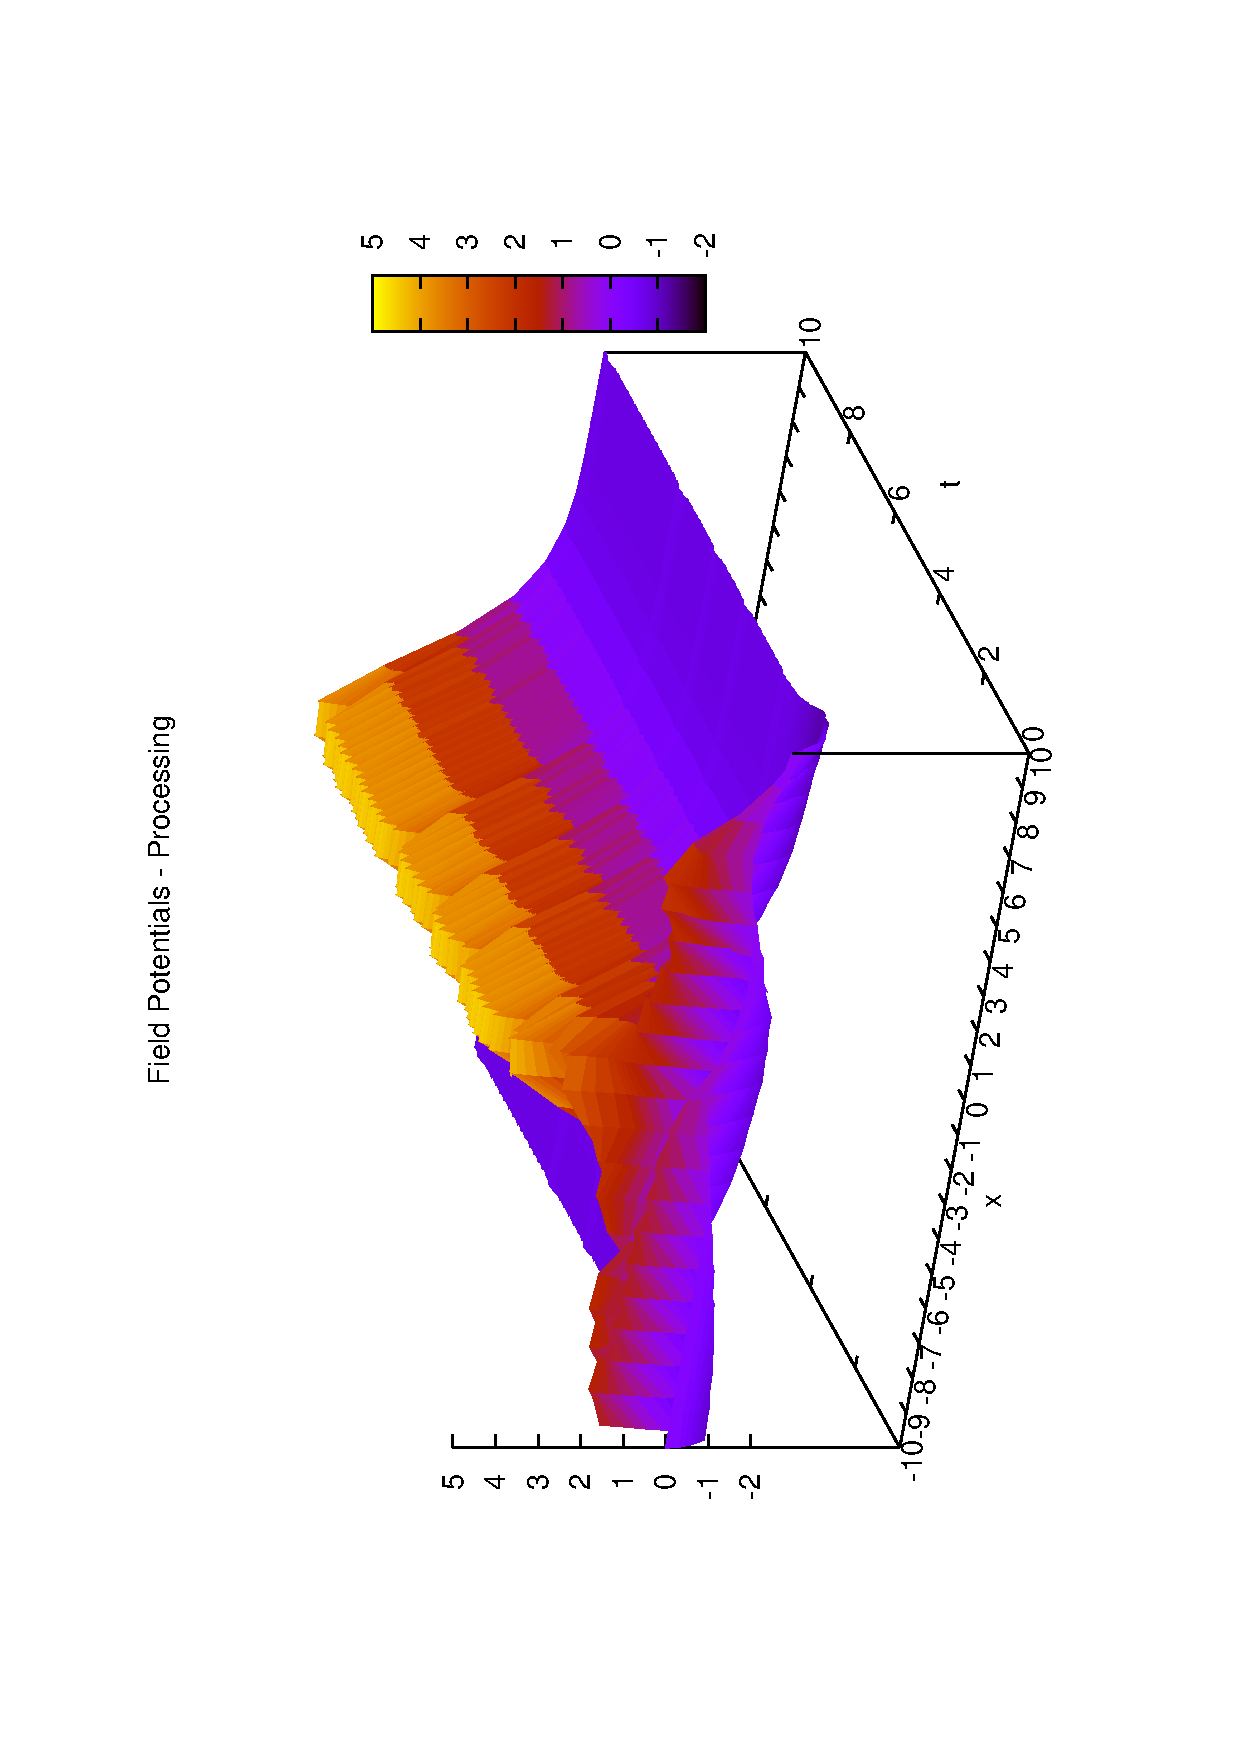
\includegraphics[angle=-90,width=7cm]{chp2-ijcnn-fieldPopulation_ijcnn}
%   \caption{Processing fields simulations between $t=0$s and $t=10$s
%   with steps $h=1/40$s and positions between $x_{min}=-10$ and
%   $x_{max}=10$. In the top, the input field architecture activation
%   is displayed (this activation is shown for comparing purposes but
%   it is not actually used by this controller). In the bottom, the
%   processing field architecture activation is displayed (actually
%   used by this controller).}
%   \label{fig:nf-activation}
% \end{figure}

\begin{figure}[p]
  \centering
  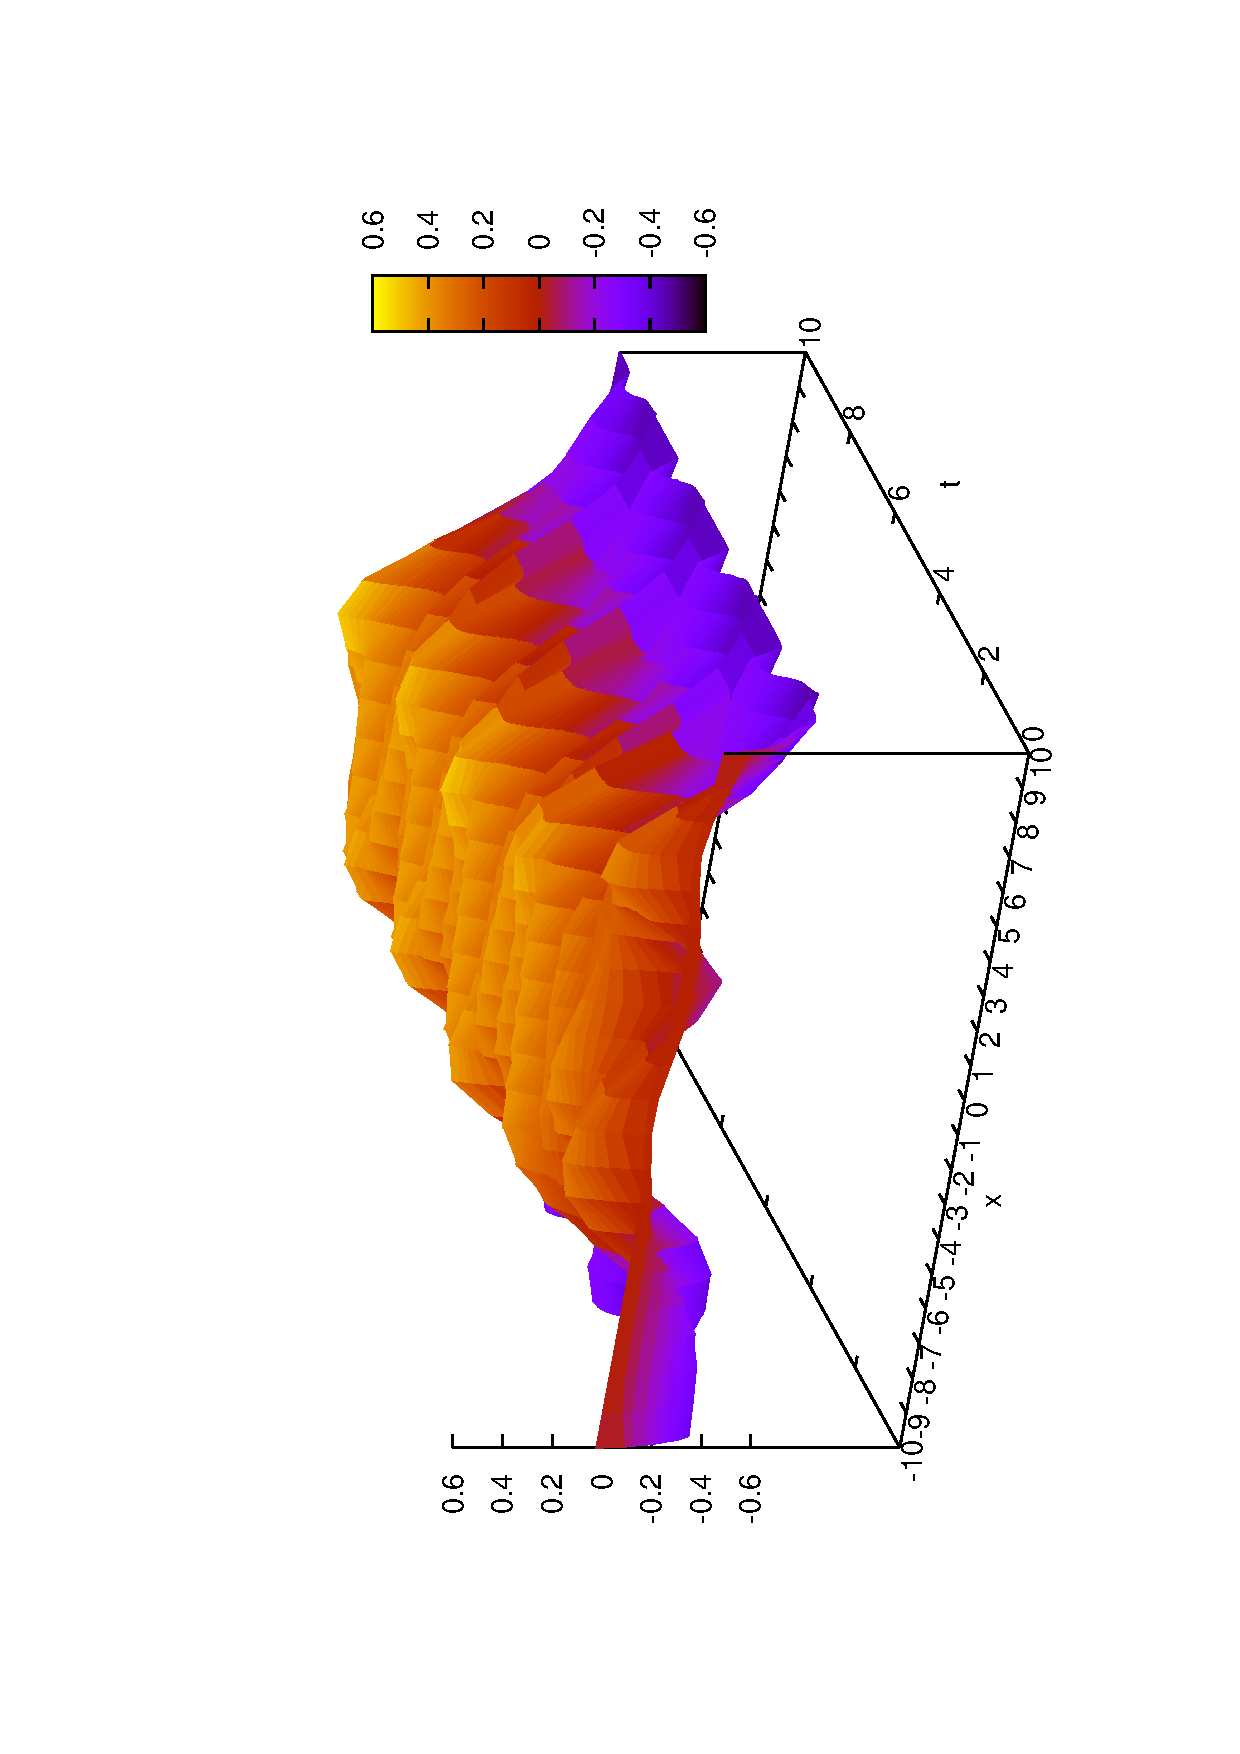
\includegraphics[width=6cm,
  angle=-90]{chp2-gecco-fieldPopulation_old}
  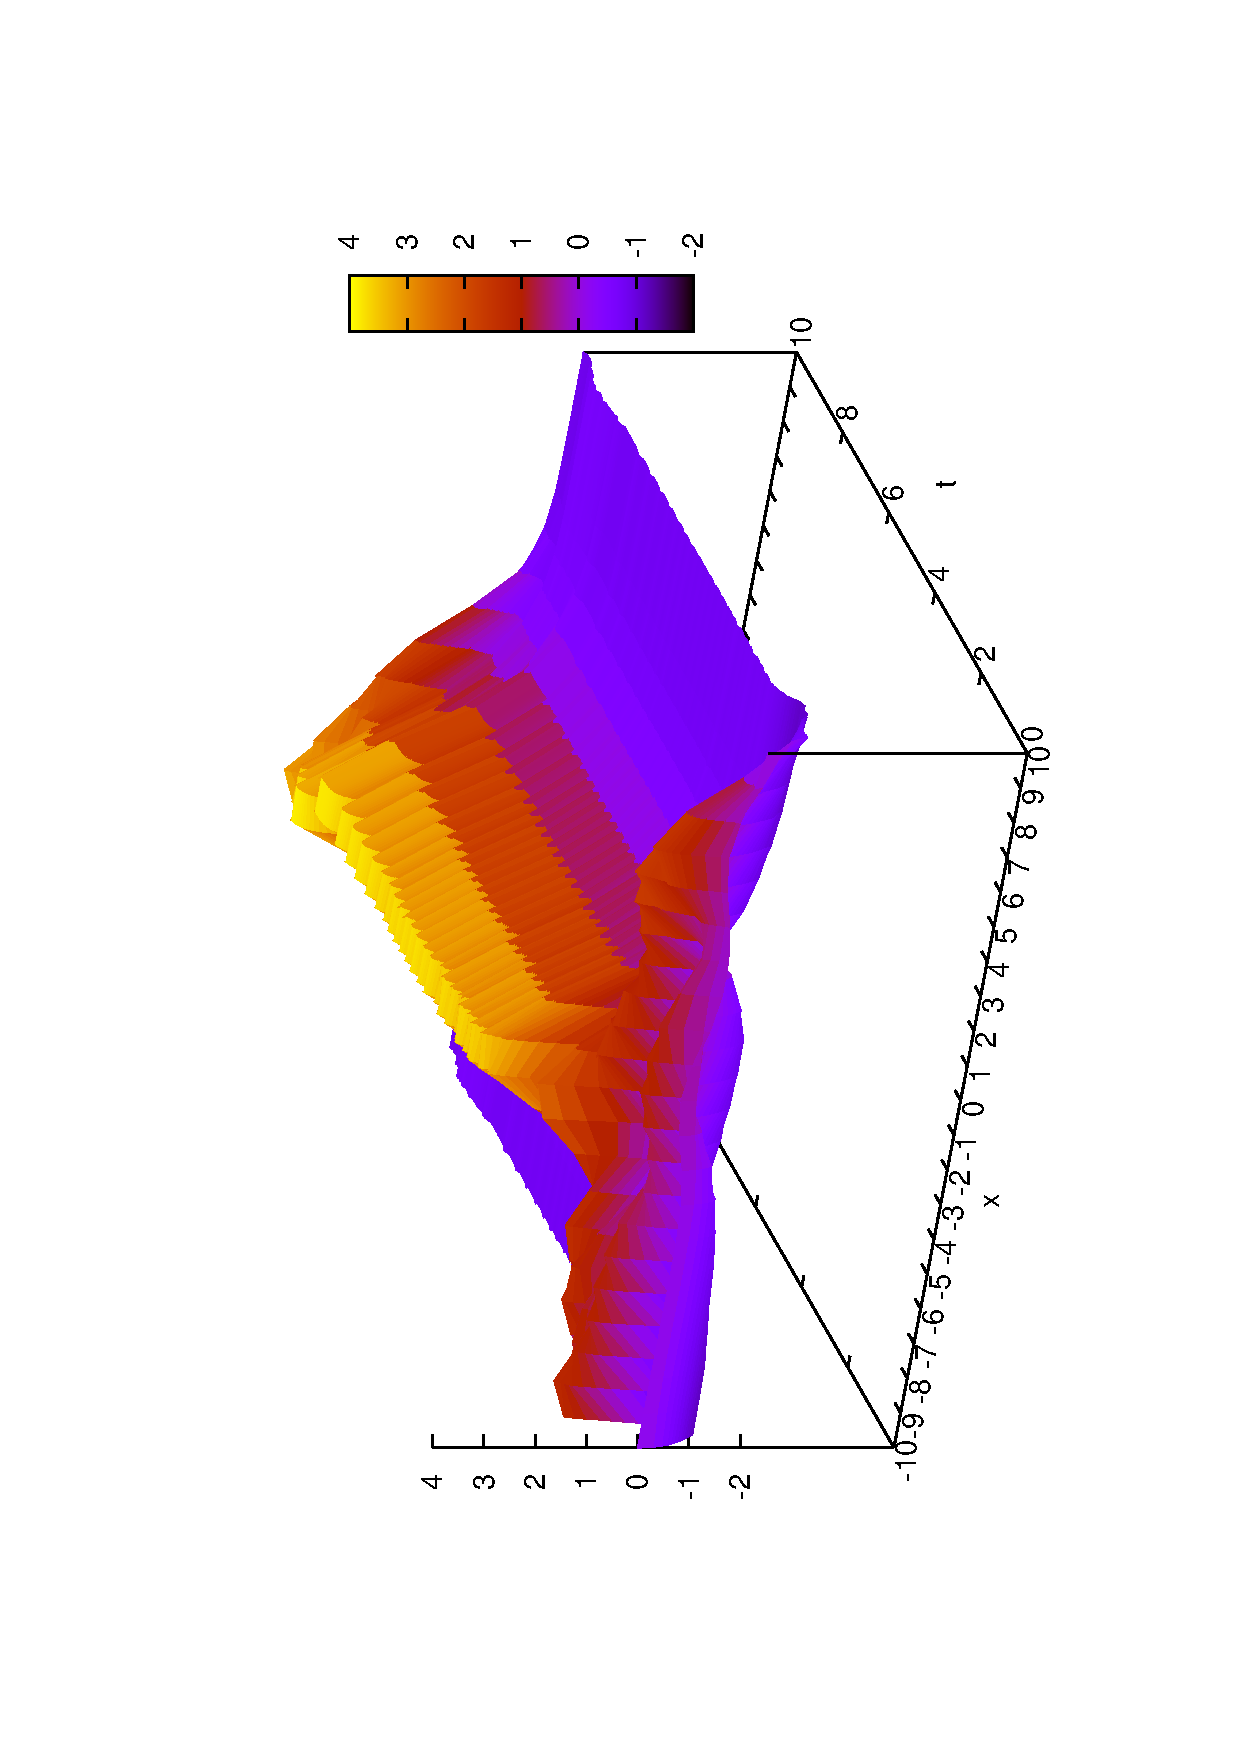
\includegraphics[width=6cm, angle=-90]{chp2-gecco-fieldPopulation}
  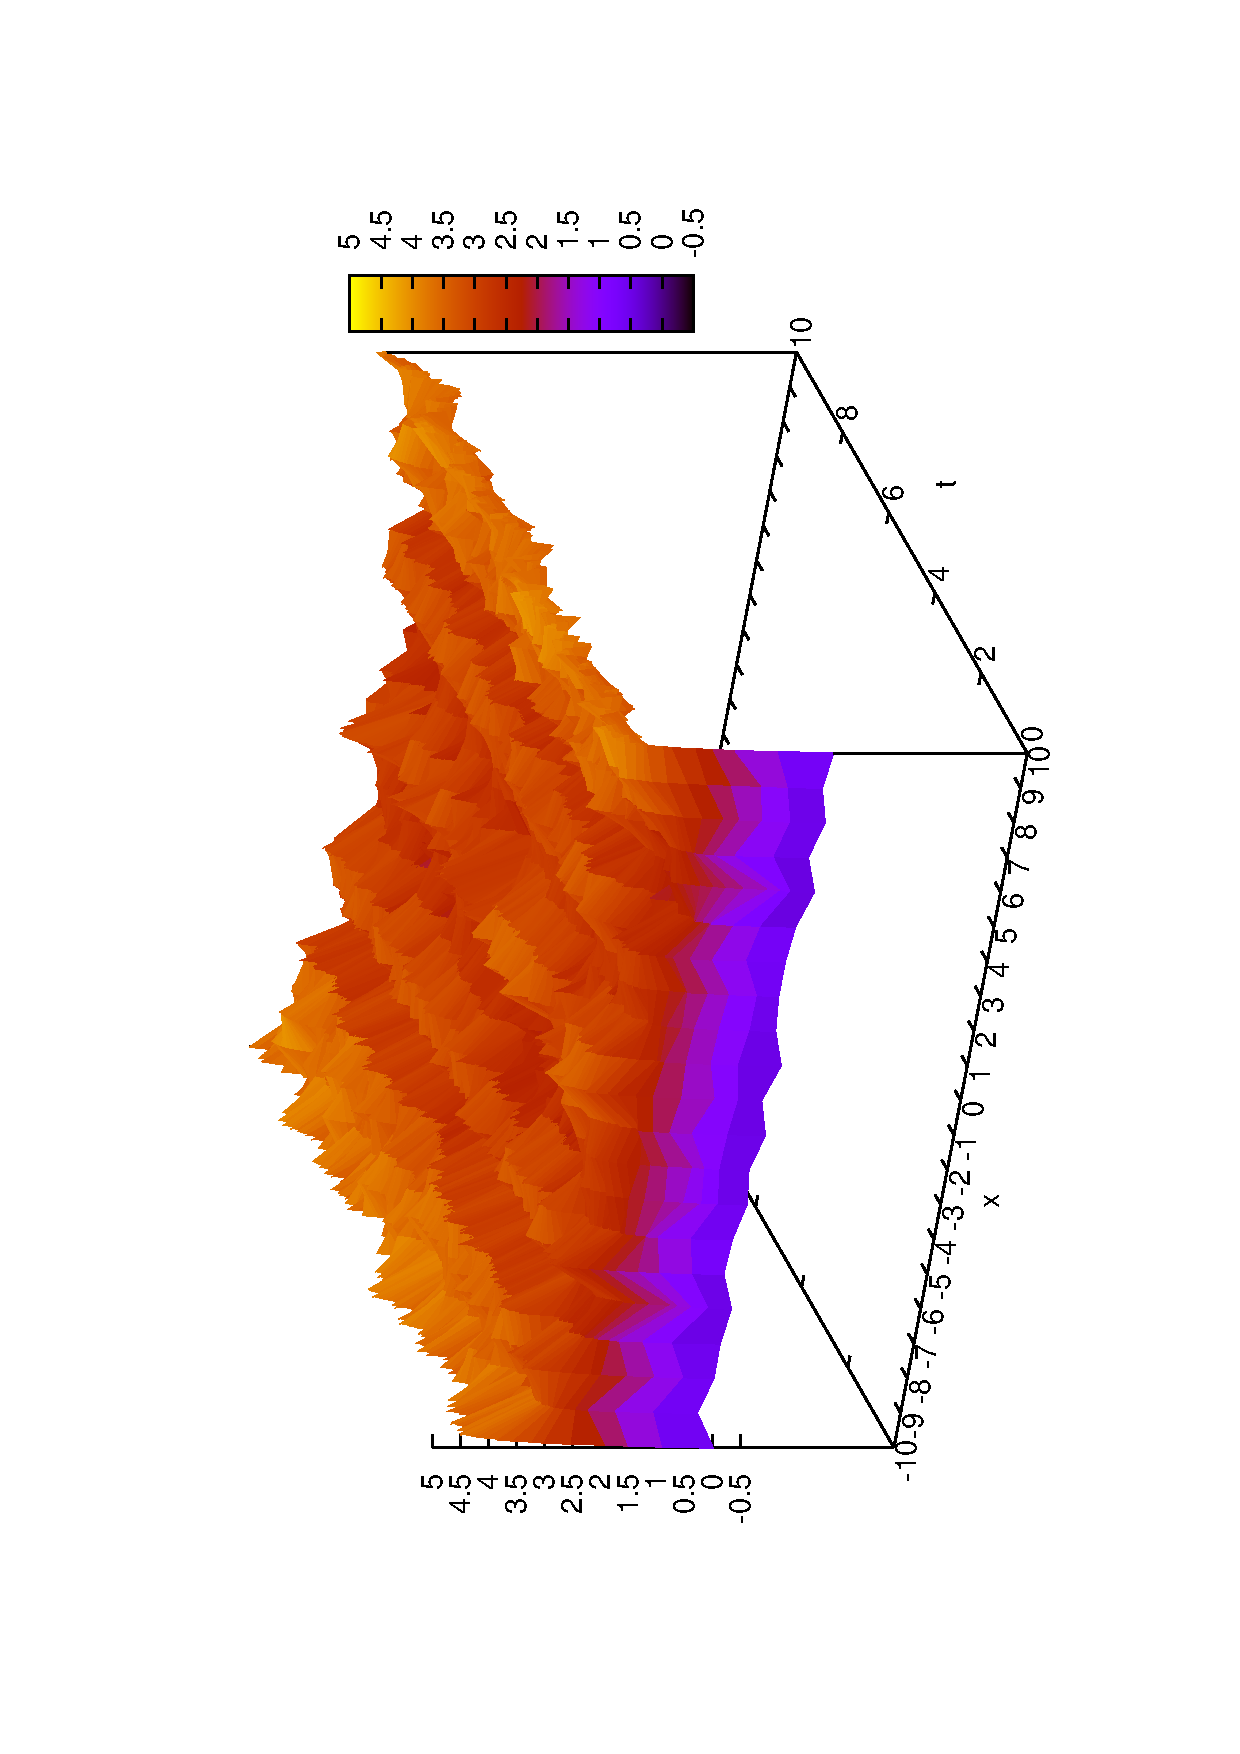
\includegraphics[width=6cm,
  angle=-90]{chp2-gecco-fieldPopulation_evo}
  \caption{Processing layer activation for simulations between $t=0$s
    and $t=10$s with steps $h=1/40$s and positions between
    $x_{min}=-10$ and $x_{max}=10$. First: direct (output from input
    layer) controller, illustrative of field dynamics excluded of the
    control action. Second: non-evolved controller. Third: evolved
    controller.}
  \label{fig:processings}
\end{figure}


\begin{figure}
  \centering
  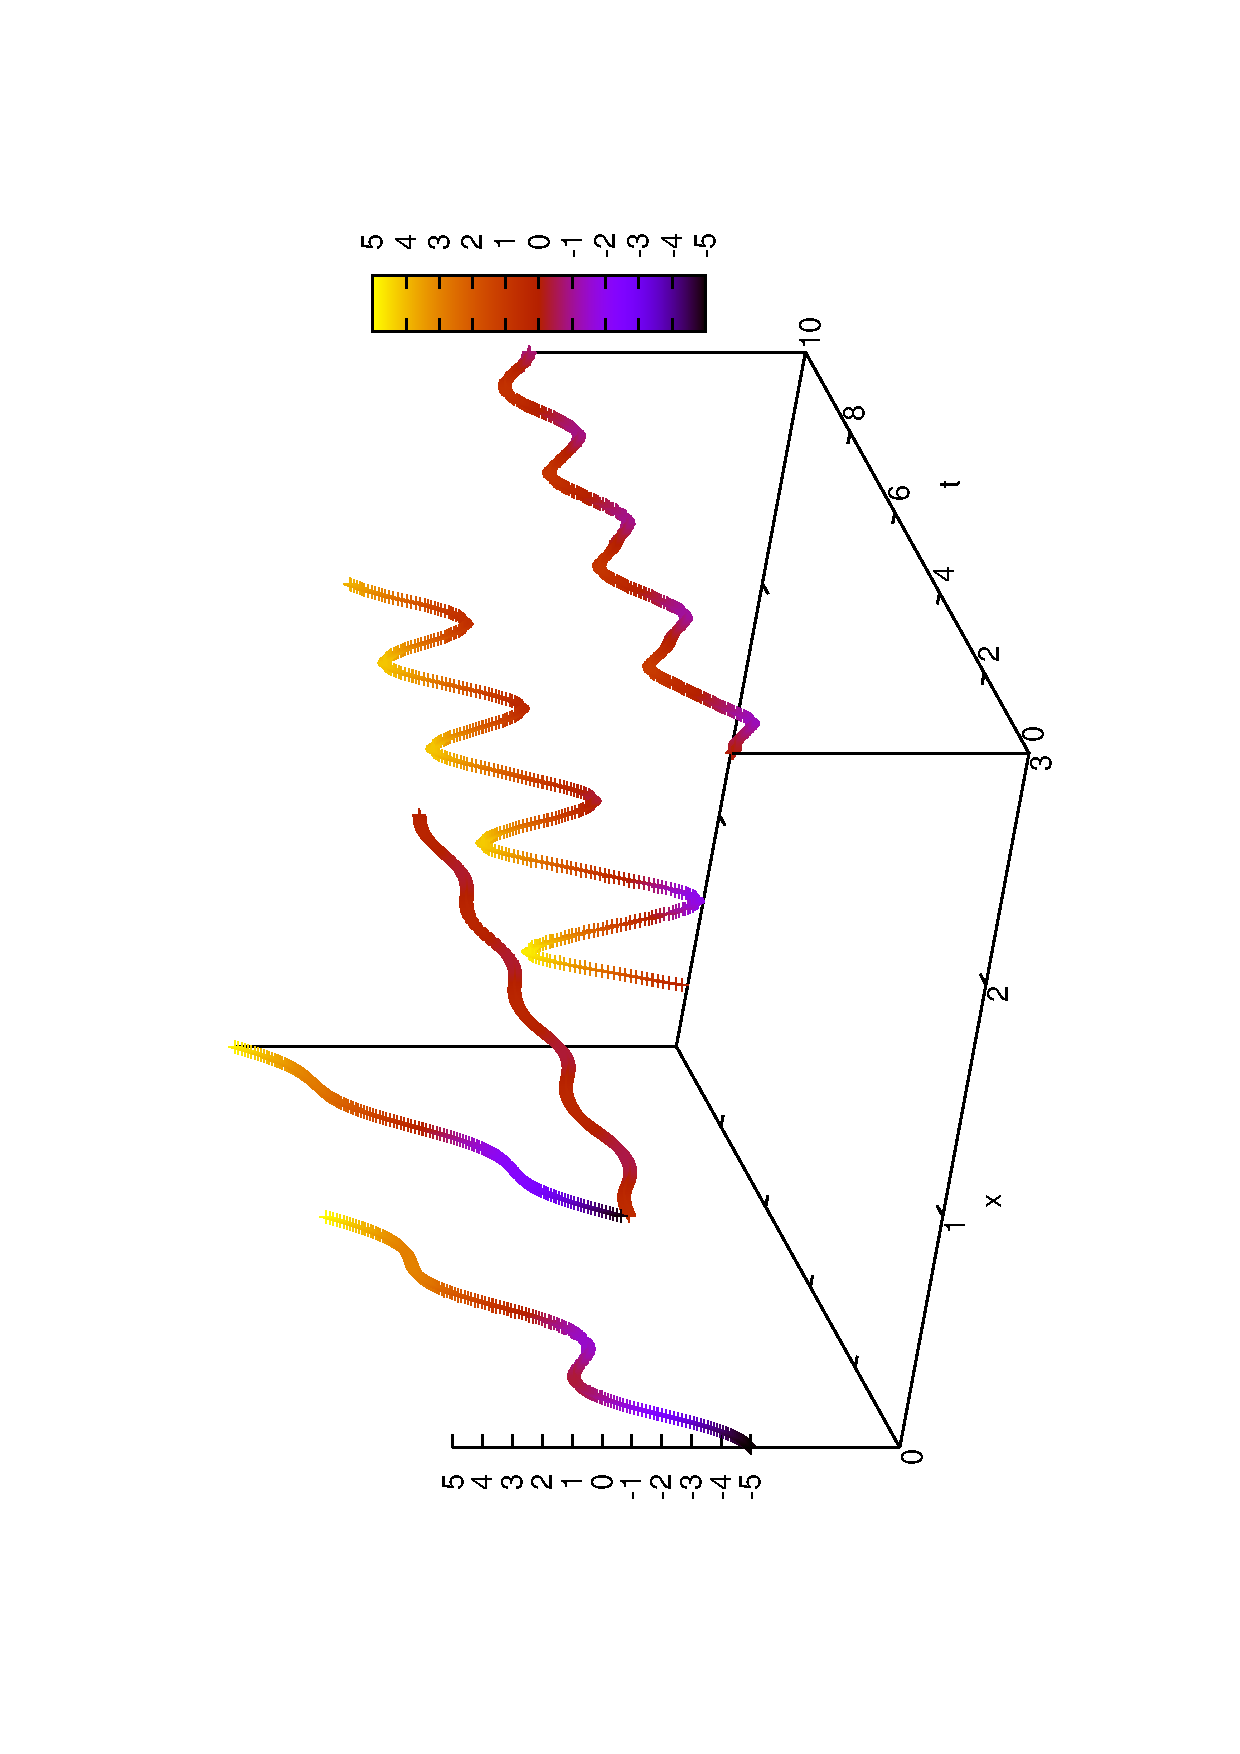
\includegraphics[width=6.5cm, angle=-90]{chp2-gecco-pendulum_old}
  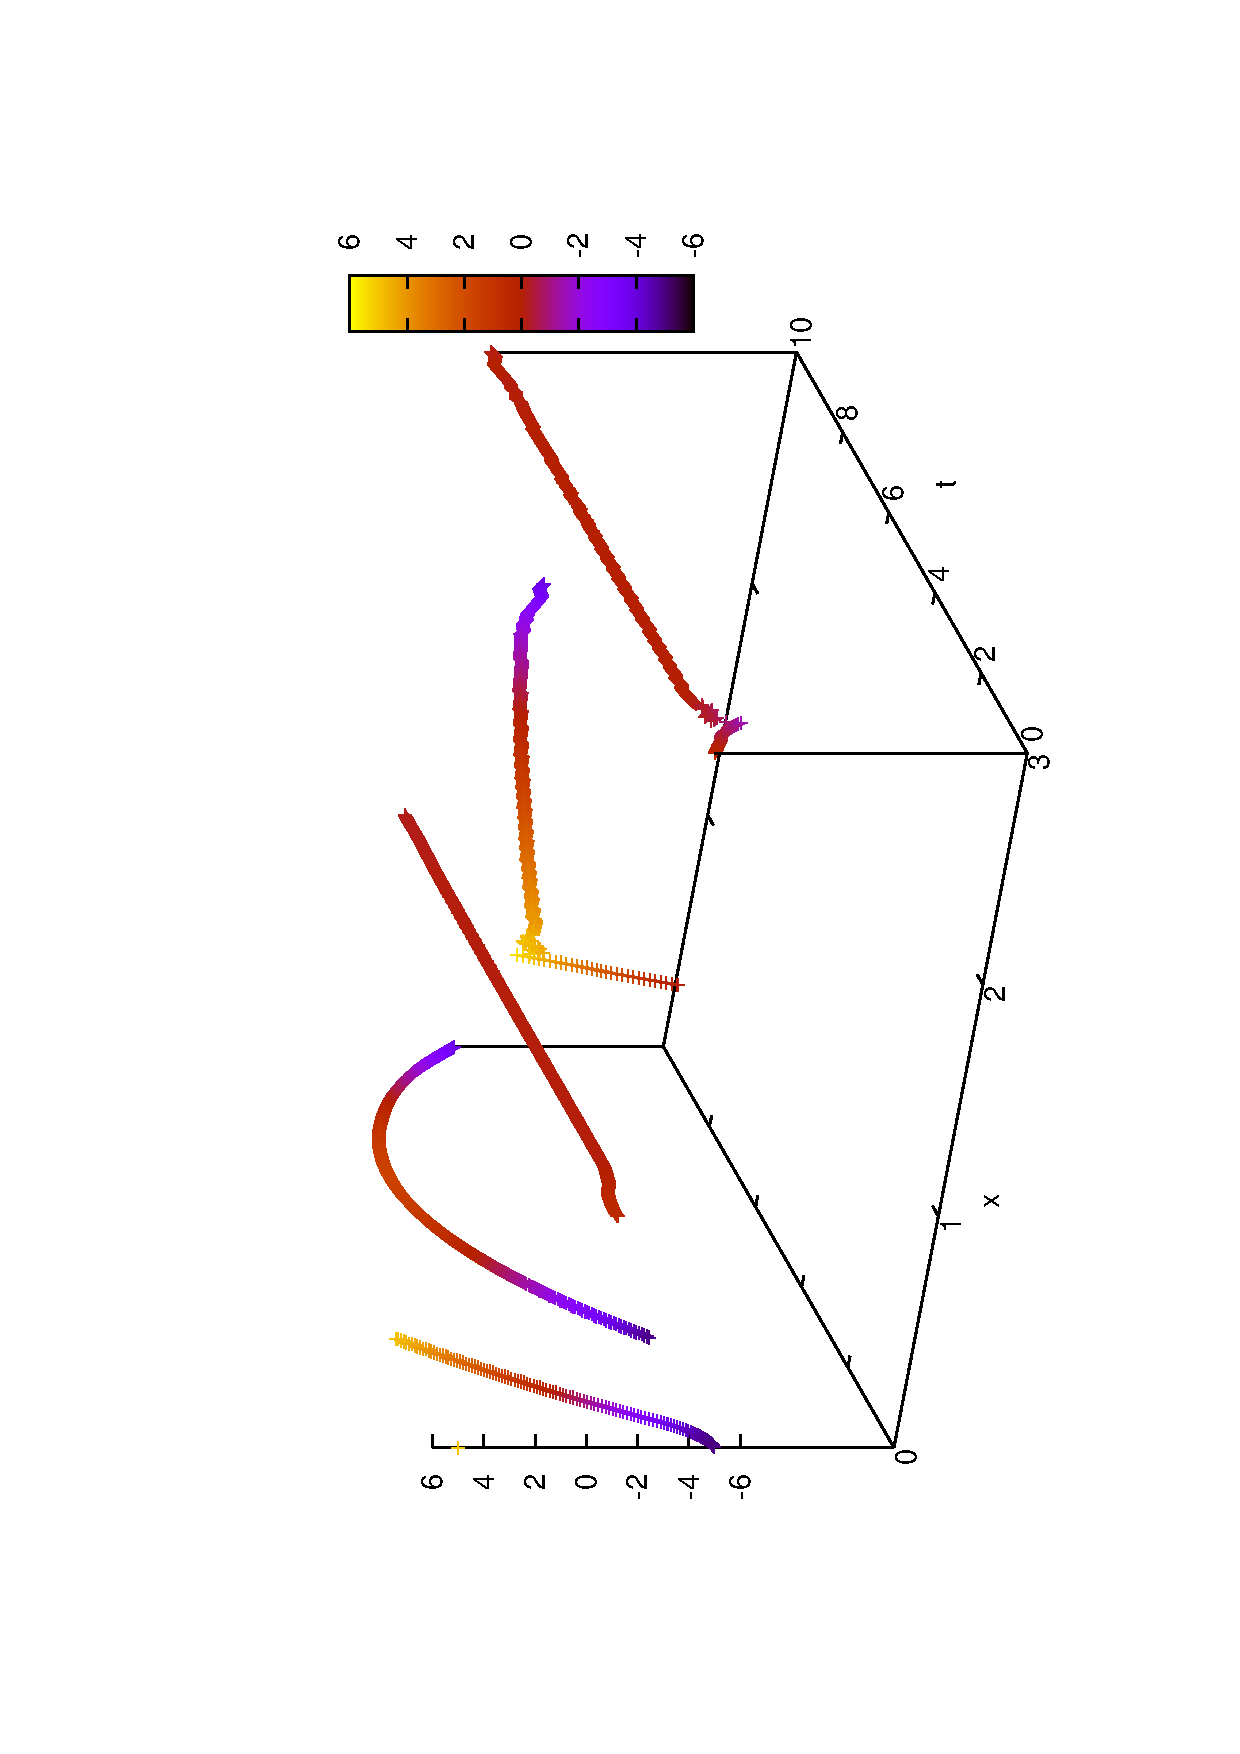
\includegraphics[width=6.5cm, angle=-90]{chp2-gecco-pendulum}
  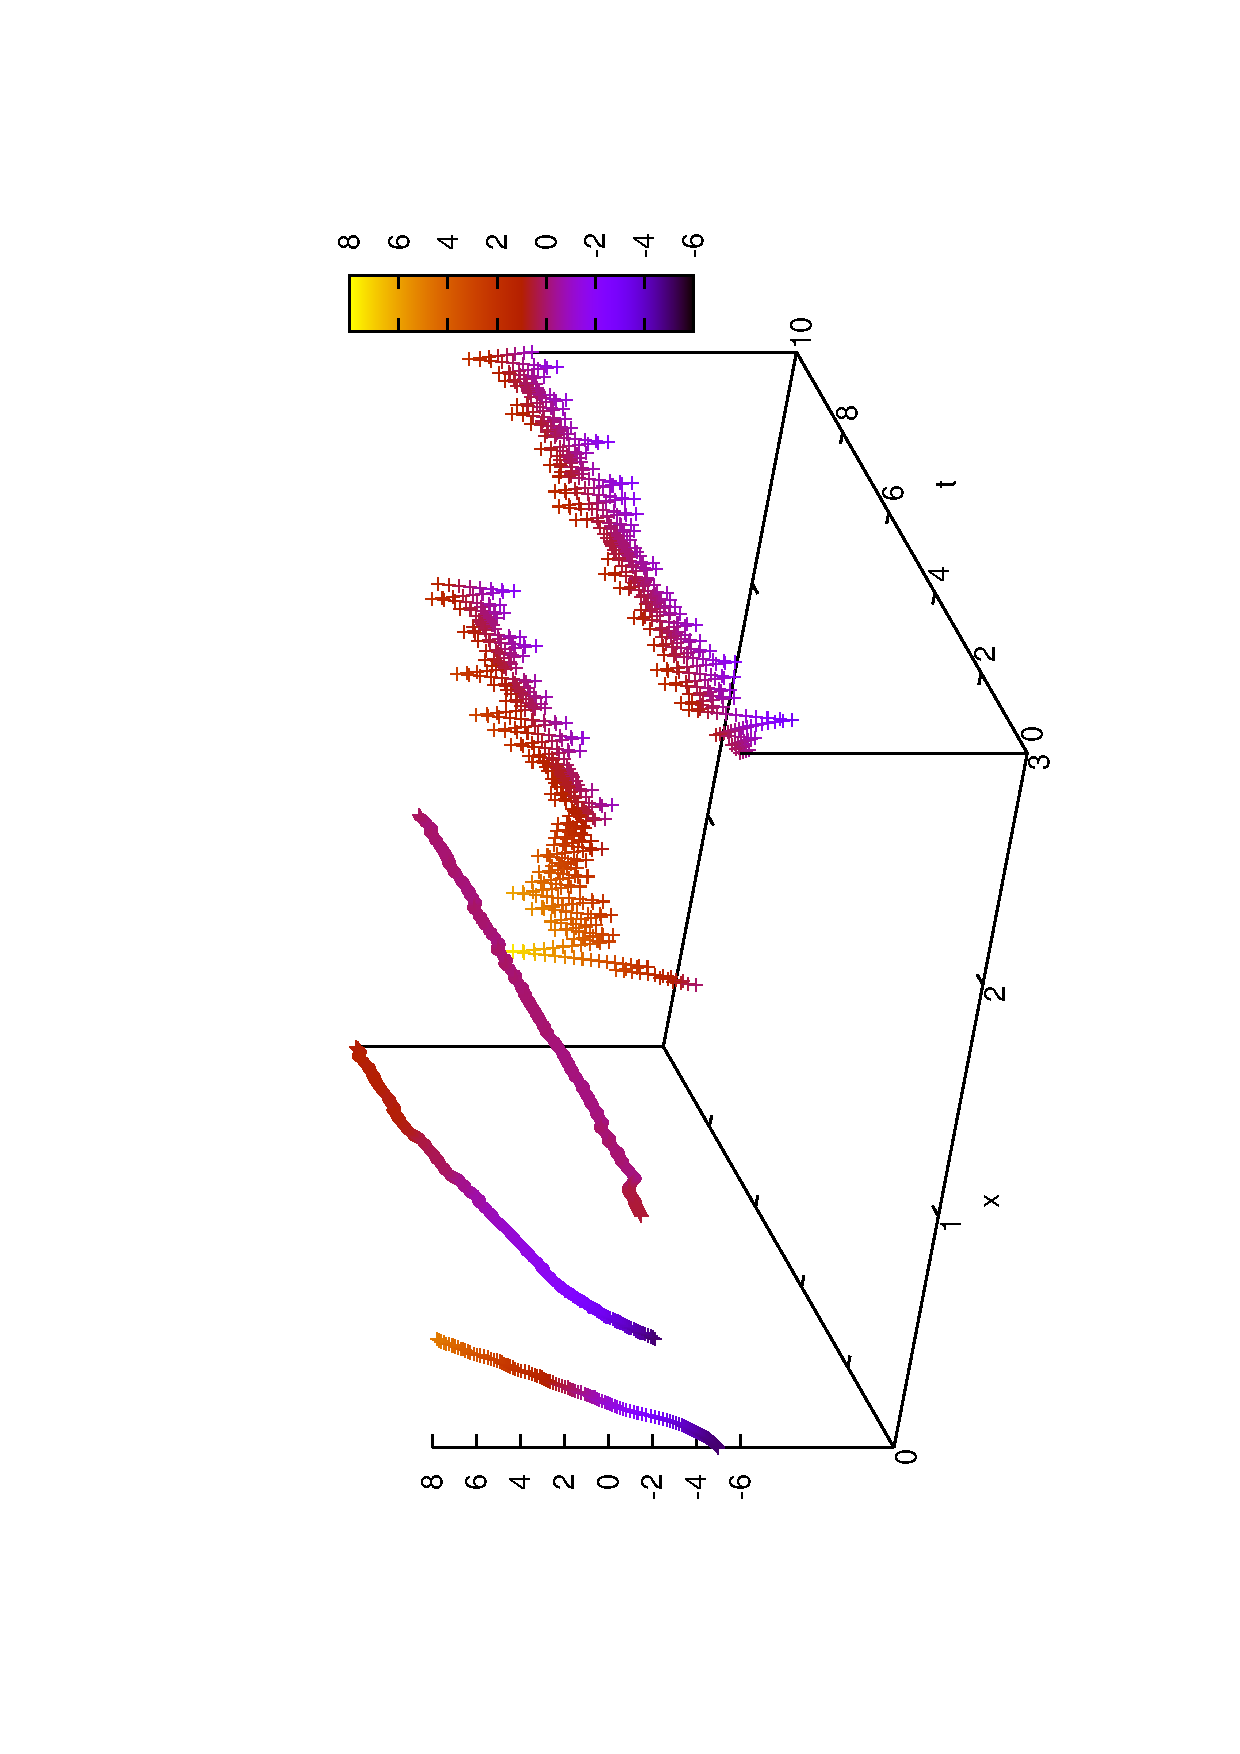
\includegraphics[width=6.5cm, angle=-90]{chp2-gecco-pendulum_evo}
  \caption{Pendulum simulation states with several neural field
    controllers between $t=0$s and $t=10$. Each state is coded with a
    position (so that the pendulum can be simulated as a field on its
    own) this way: $x$:0, $\theta$:1, $\dot{x}$:2,
    $\dot{\theta}$:3. It can be seen the little variation in the
    angular position ($\theta$). The discontinuity in $x$ is present
    because position wraps in the simulation so that $x=5$ is
    equivalent to $x=-5$. First: direct (without processing layer)
    controller. Second: non-evolved controller. Third: evolved
    controller.}
  \label{fig:pendulum-states}
\end{figure}


\section{Discussion}
The results obtained from this chapter can be summarized in a short
analysis.

While the recurrent neural network controller is expressive enough to
solve the problem at hand, the number of parameters to configure (or
in this case to evolve) is of a quadratic order in relation to the
number of nodes (or neurons). This was not a particular problem for
the evolutionary algorithm used, but limits its potential
scalability. Furthermore, while it is expressive enough, does not show
a particular suitability to the dynamic stability problem of the
inverted pendulum and there are no reasons to expect something
different for a more complex biped model.

On the other hand, the neural field controller is a bit more complex
and its simulation more costly, but has some notable advantages. The
first one is its ability to self-compensate or, equivalently, the
stability of its natural dynamics, which is attained after the setup
of few parameters. The second one is it suitability to the problem at
hand, being able to solve it with a acceptable degree of performance
for low and mid perturbations without evolution.

Although there was a need for parameter configuration to attain a good
performance, evolution was not strictly required because the small
number of parameters to setup: basically three parameters of the
kernel function and the resting potential of the field equation, a
number of parameters of constant order in relation to the number of
nodes (discrete potentials on the neural field). Nonetheless, the
evolved controller performed better than the other two, is more
general because eliminates the need for manual conscious
parametrization and allows the designer to specify more precisely the
performance measure desired.

It is worth noting that the neural field has a spatial representation
which allows interpretation of field potentials (as shown in
fig. \ref{fig:processings}). Indeed, its geometrical representation
allows for a small switch between a state-space like controller to a
neural field controller. The interpretation or understanding of
recurrent neural networks tends to be difficult and even more with
increasing states involved. This makes the neural field controller not
as black-box as the a recurrent neural network controller. This holds
even in the case of the evolved neural field controller.

More complex control problems could benefit from the strategy of
parametrization of neural field controllers by evolution here
developed. This way, it is left for future work the task of
integration of multiple goals in different populations and the design
of an arbitration scheme compatible with the architecture.

While the cart-and-pole biped walking model is useful as a first
approach to the problem of locomotion, in order to develop a more
realistic controller of biped walking, a model closer to human biped
walking will be explored in the next chapter, and also some new
controllers will be presented.








